\documentclass[review]{elsarticle}

\usepackage{lineno}
\usepackage{xspace}
\modulolinenumbers[5]

\journal{Annals of Nuclear Energy}

%% `Elsevier LaTeX' style
\bibliographystyle{elsarticle-num}
%%%%%%%%%%%%%%%%%%%%%%%

%%%% packages and definitions (optional)
\usepackage{placeins}
\usepackage{booktabs} % nice rules (thick lines) for tables
\usepackage{microtype} % improves typography for PDF
\usepackage{hhline}
\usepackage{amsmath}

%\usepackage[demo]{graphicx}
%\usepackage{caption}
%\usepackage{subcaption}

\usepackage{booktabs}
\usepackage{threeparttable, tablefootnote}

\usepackage{tabularx}
\newcolumntype{b}{>{\hsize=1.0\hsize}X}
\newcolumntype{s}{>{\hsize=.5\hsize}X}
\newcolumntype{m}{>{\hsize=.75\hsize}X}
\newcolumntype{x}{>{\hsize=.25\hsize}X}

%\newcommand{\Cyclus}{\textsc{Cyclus}\xspace}%
%\newcommand{\Cycamore}{\textsc{Cycamore}\xspace}%
\graphicspath{ {../figures/} }

% tikz %
\usepackage{tikz}
\usetikzlibrary{positioning, arrows, decorations, shapes}

\usetikzlibrary{shapes.geometric,arrows}
\tikzstyle{process} = [rectangle, rounded corners, minimum width=3cm, minimum height=1cm,text centered, draw=black, fill=blue!30]
\tikzstyle{object} = [ellipse, rounded corners, minimum width=3cm, minimum height=1cm,text centered, draw=black, fill=green!30]
\tikzstyle{arrow} = [thick,->,>=stealth]

% hyperref %
\usepackage[hidelinks]{hyperref}

\begin{document}
\begin{frontmatter}
\title{Graphical Abstract\\
Modeling and Simulation of Online Reprocessing in the Thorium-Fueled Molten Salt Breeder Reactor}
\date{}                     %% if you don't need date to appear

\end{frontmatter}

\begin{figure}[htbp!]
    \begin{center}
        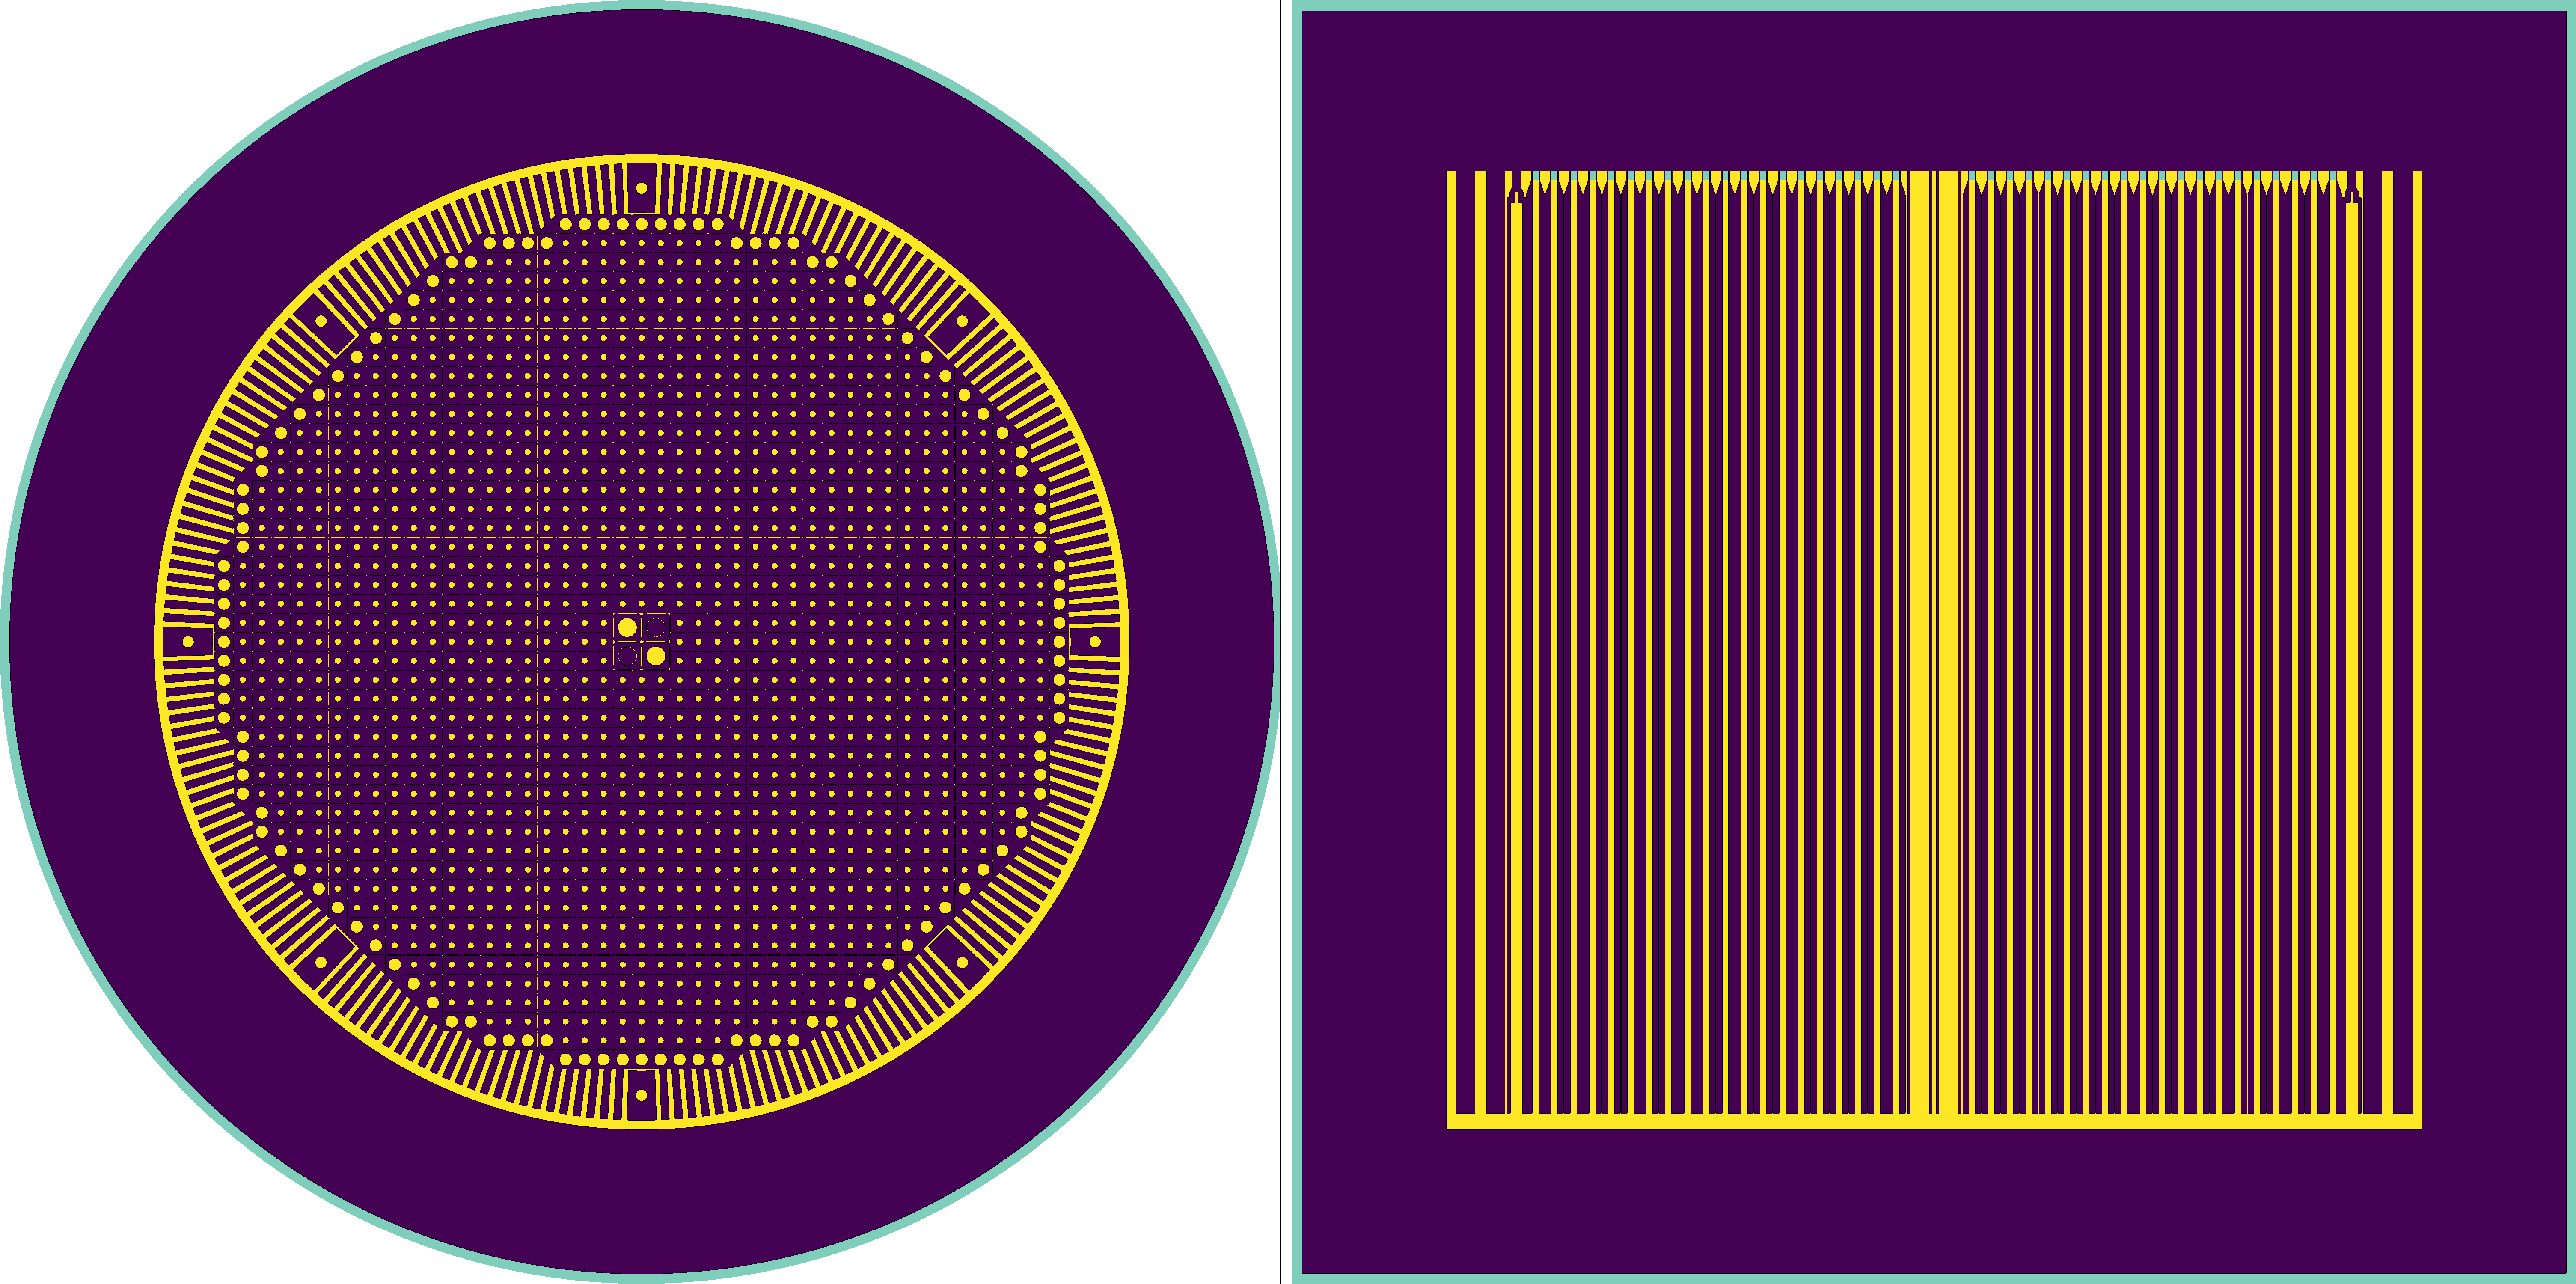
\includegraphics[width=\textwidth]{view_serpent.png}
    \end{center}
    \caption{Plan and elevation views of SERPENT 2 Molten Salt Breeder Reactor model developed in this work.}
    \label{fig:graph-abs}
\end{figure}
\begin{figure}[htbp!]
    \begin{center}
        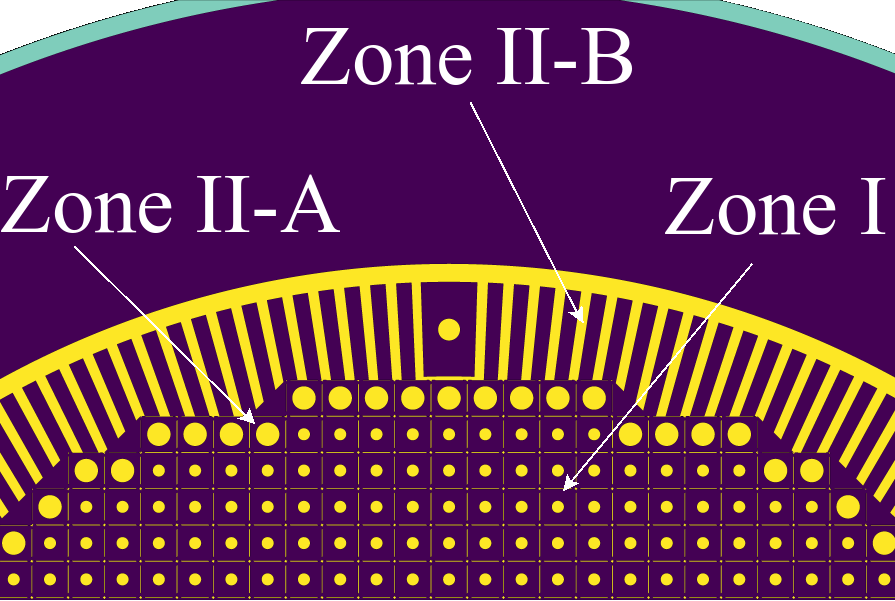
\includegraphics[width=\textwidth]{ser_zone_II.png}
    \end{center}
    \caption{Detailed view of Molten Salt Breeder Reactor zone II model.}
    \label{fig:serpent-zoneII}
\end{figure}
\begin{figure}[htbp!]
    \begin{center}
        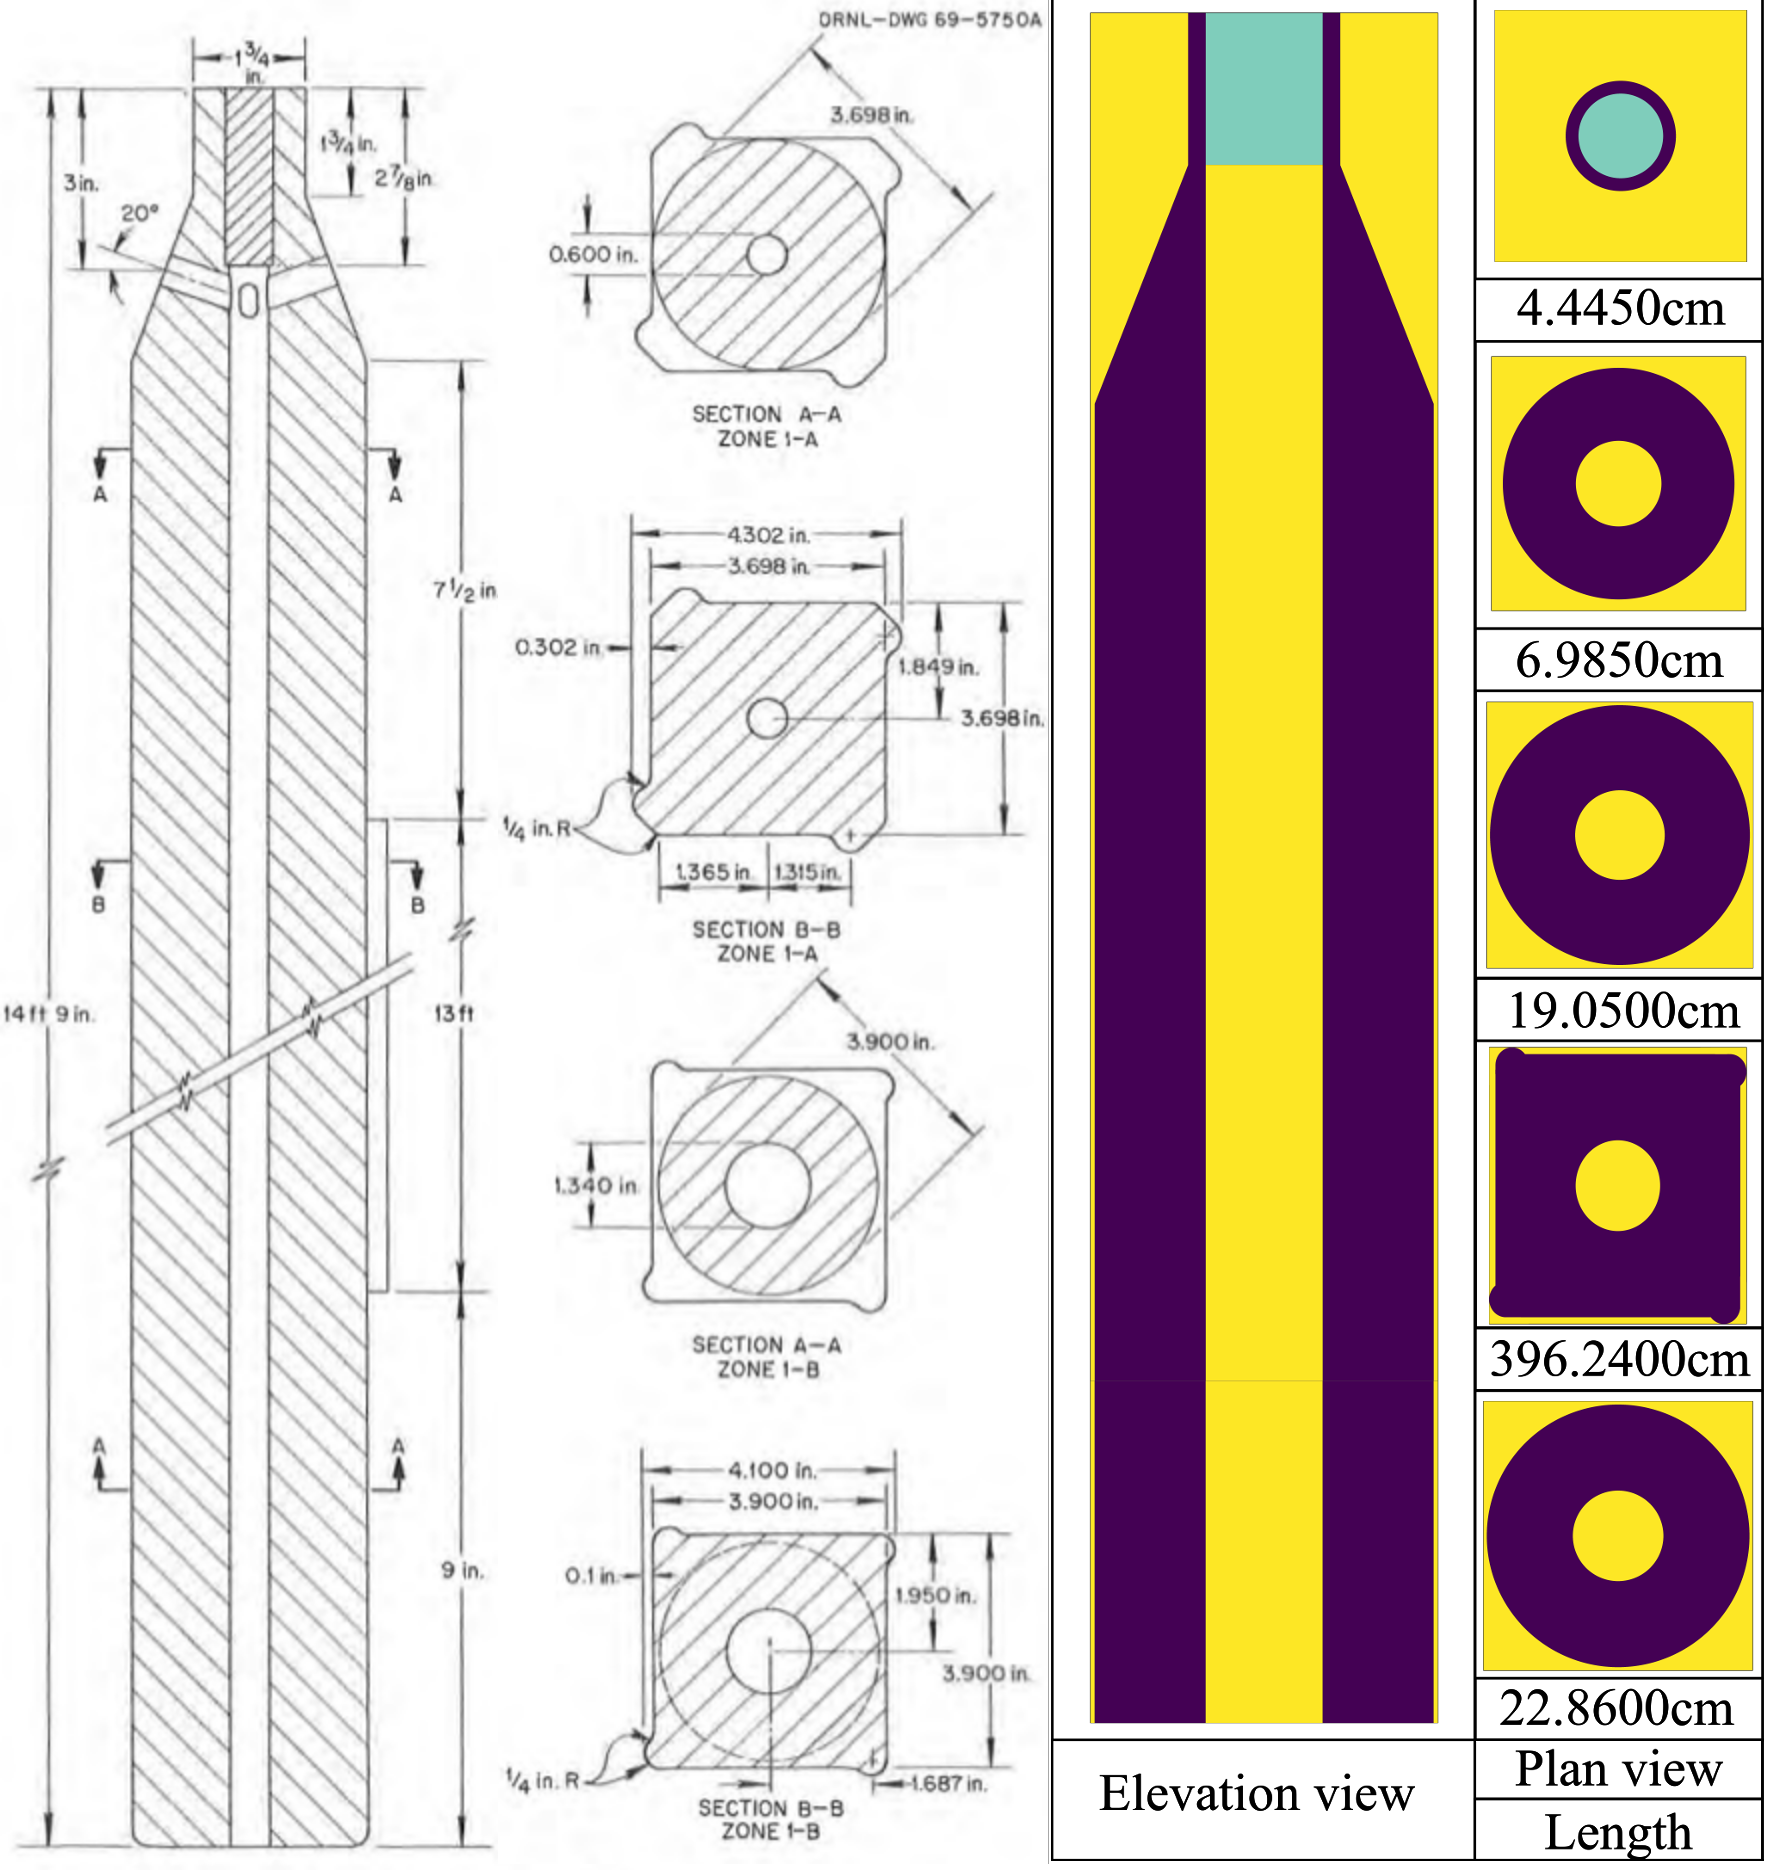
\includegraphics[width=\textwidth]{zone_I_element_ref.png}
    \end{center}
    \caption{Graphite moderator elements for zone I.}
  	\label{fig:I_element_ref}
\end{figure}
\begin{figure}[htbp!]
    \begin{center}
		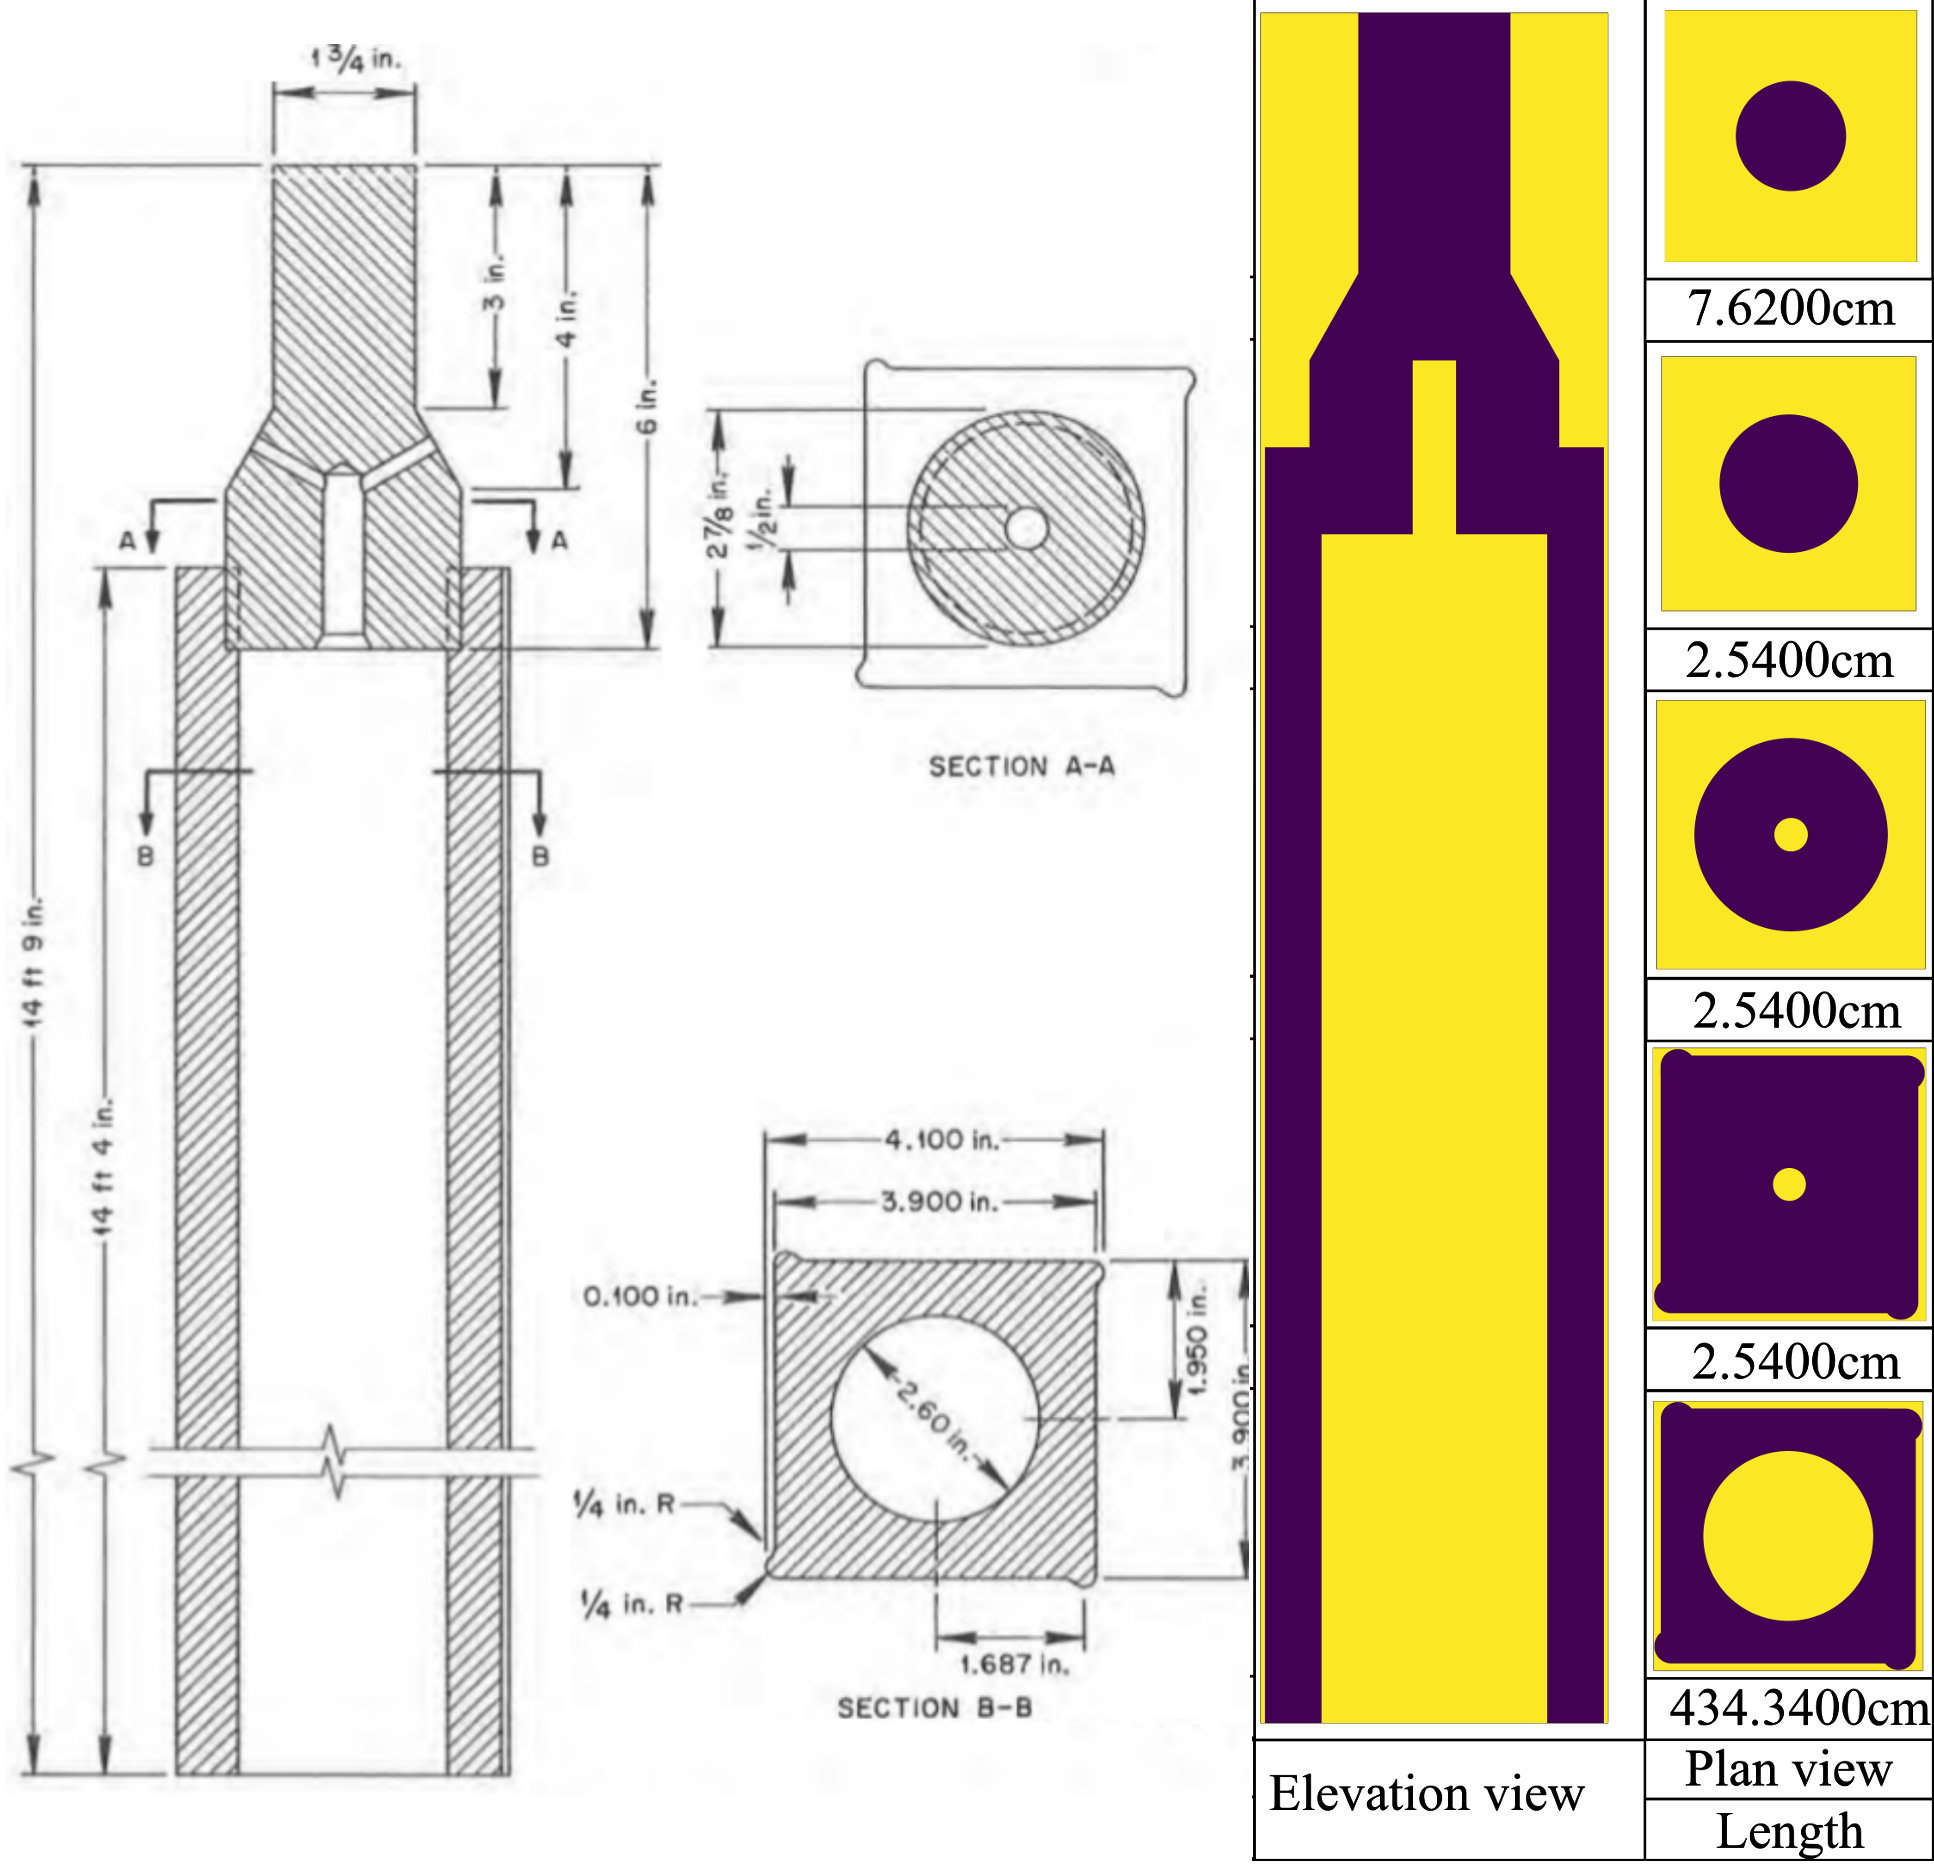
\includegraphics[width=\textwidth]{zone_II_element_ref.png}
    \end{center}
	\caption{Graphite moderator elements for zone II-A.}
	\label{fig:II_element_ref}
\end{figure}
\begin{figure}[htbp!]
    \begin{center}
		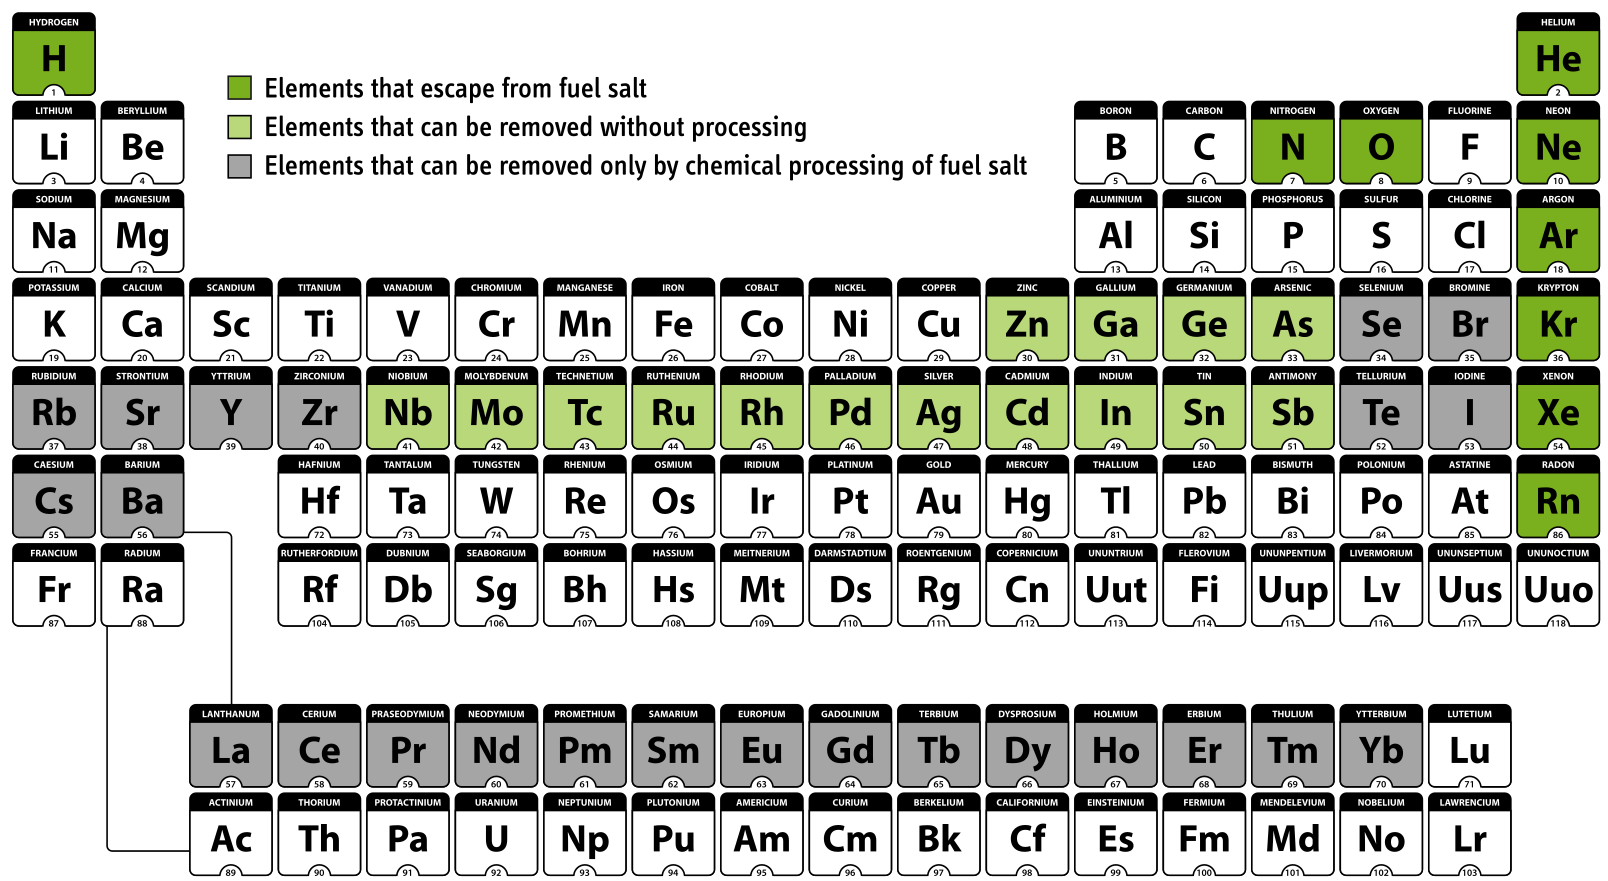
\includegraphics[width=\textwidth]{periodic_map.png}
    \end{center}
	\caption{Processing options for Molten Salt Reactor fuels.}
	\label{fig:periodic_tab}
\end{figure}
\begin{figure}[htbp!]
    \begin{center}
		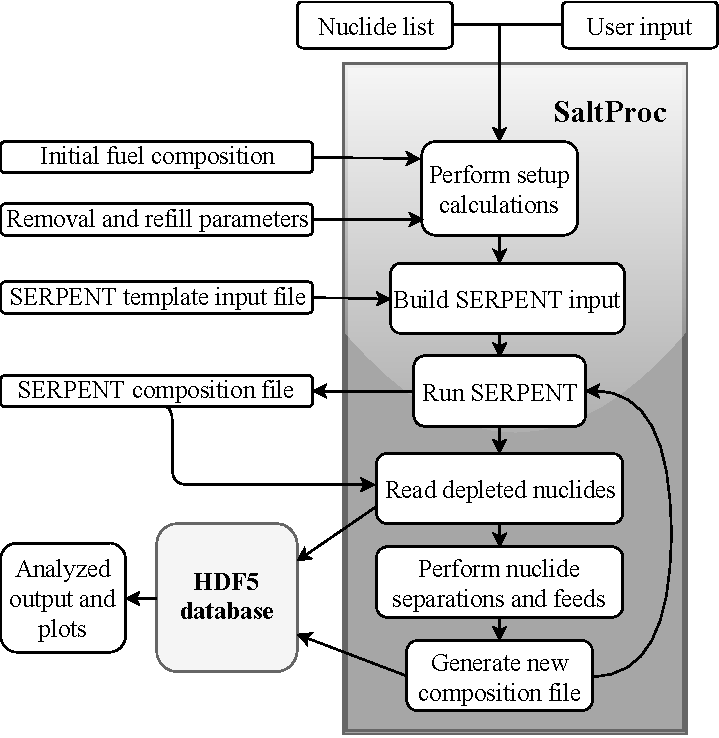
\includegraphics[width=0.75\textwidth]{saltproc_flowchart.pdf}
    \end{center}
  \caption{Flow chart for the Saltproc python-based tools.}
  \label{fig:saltproc_flow}
\end{figure}
\begin{figure}[htbp!]
    \begin{center}
		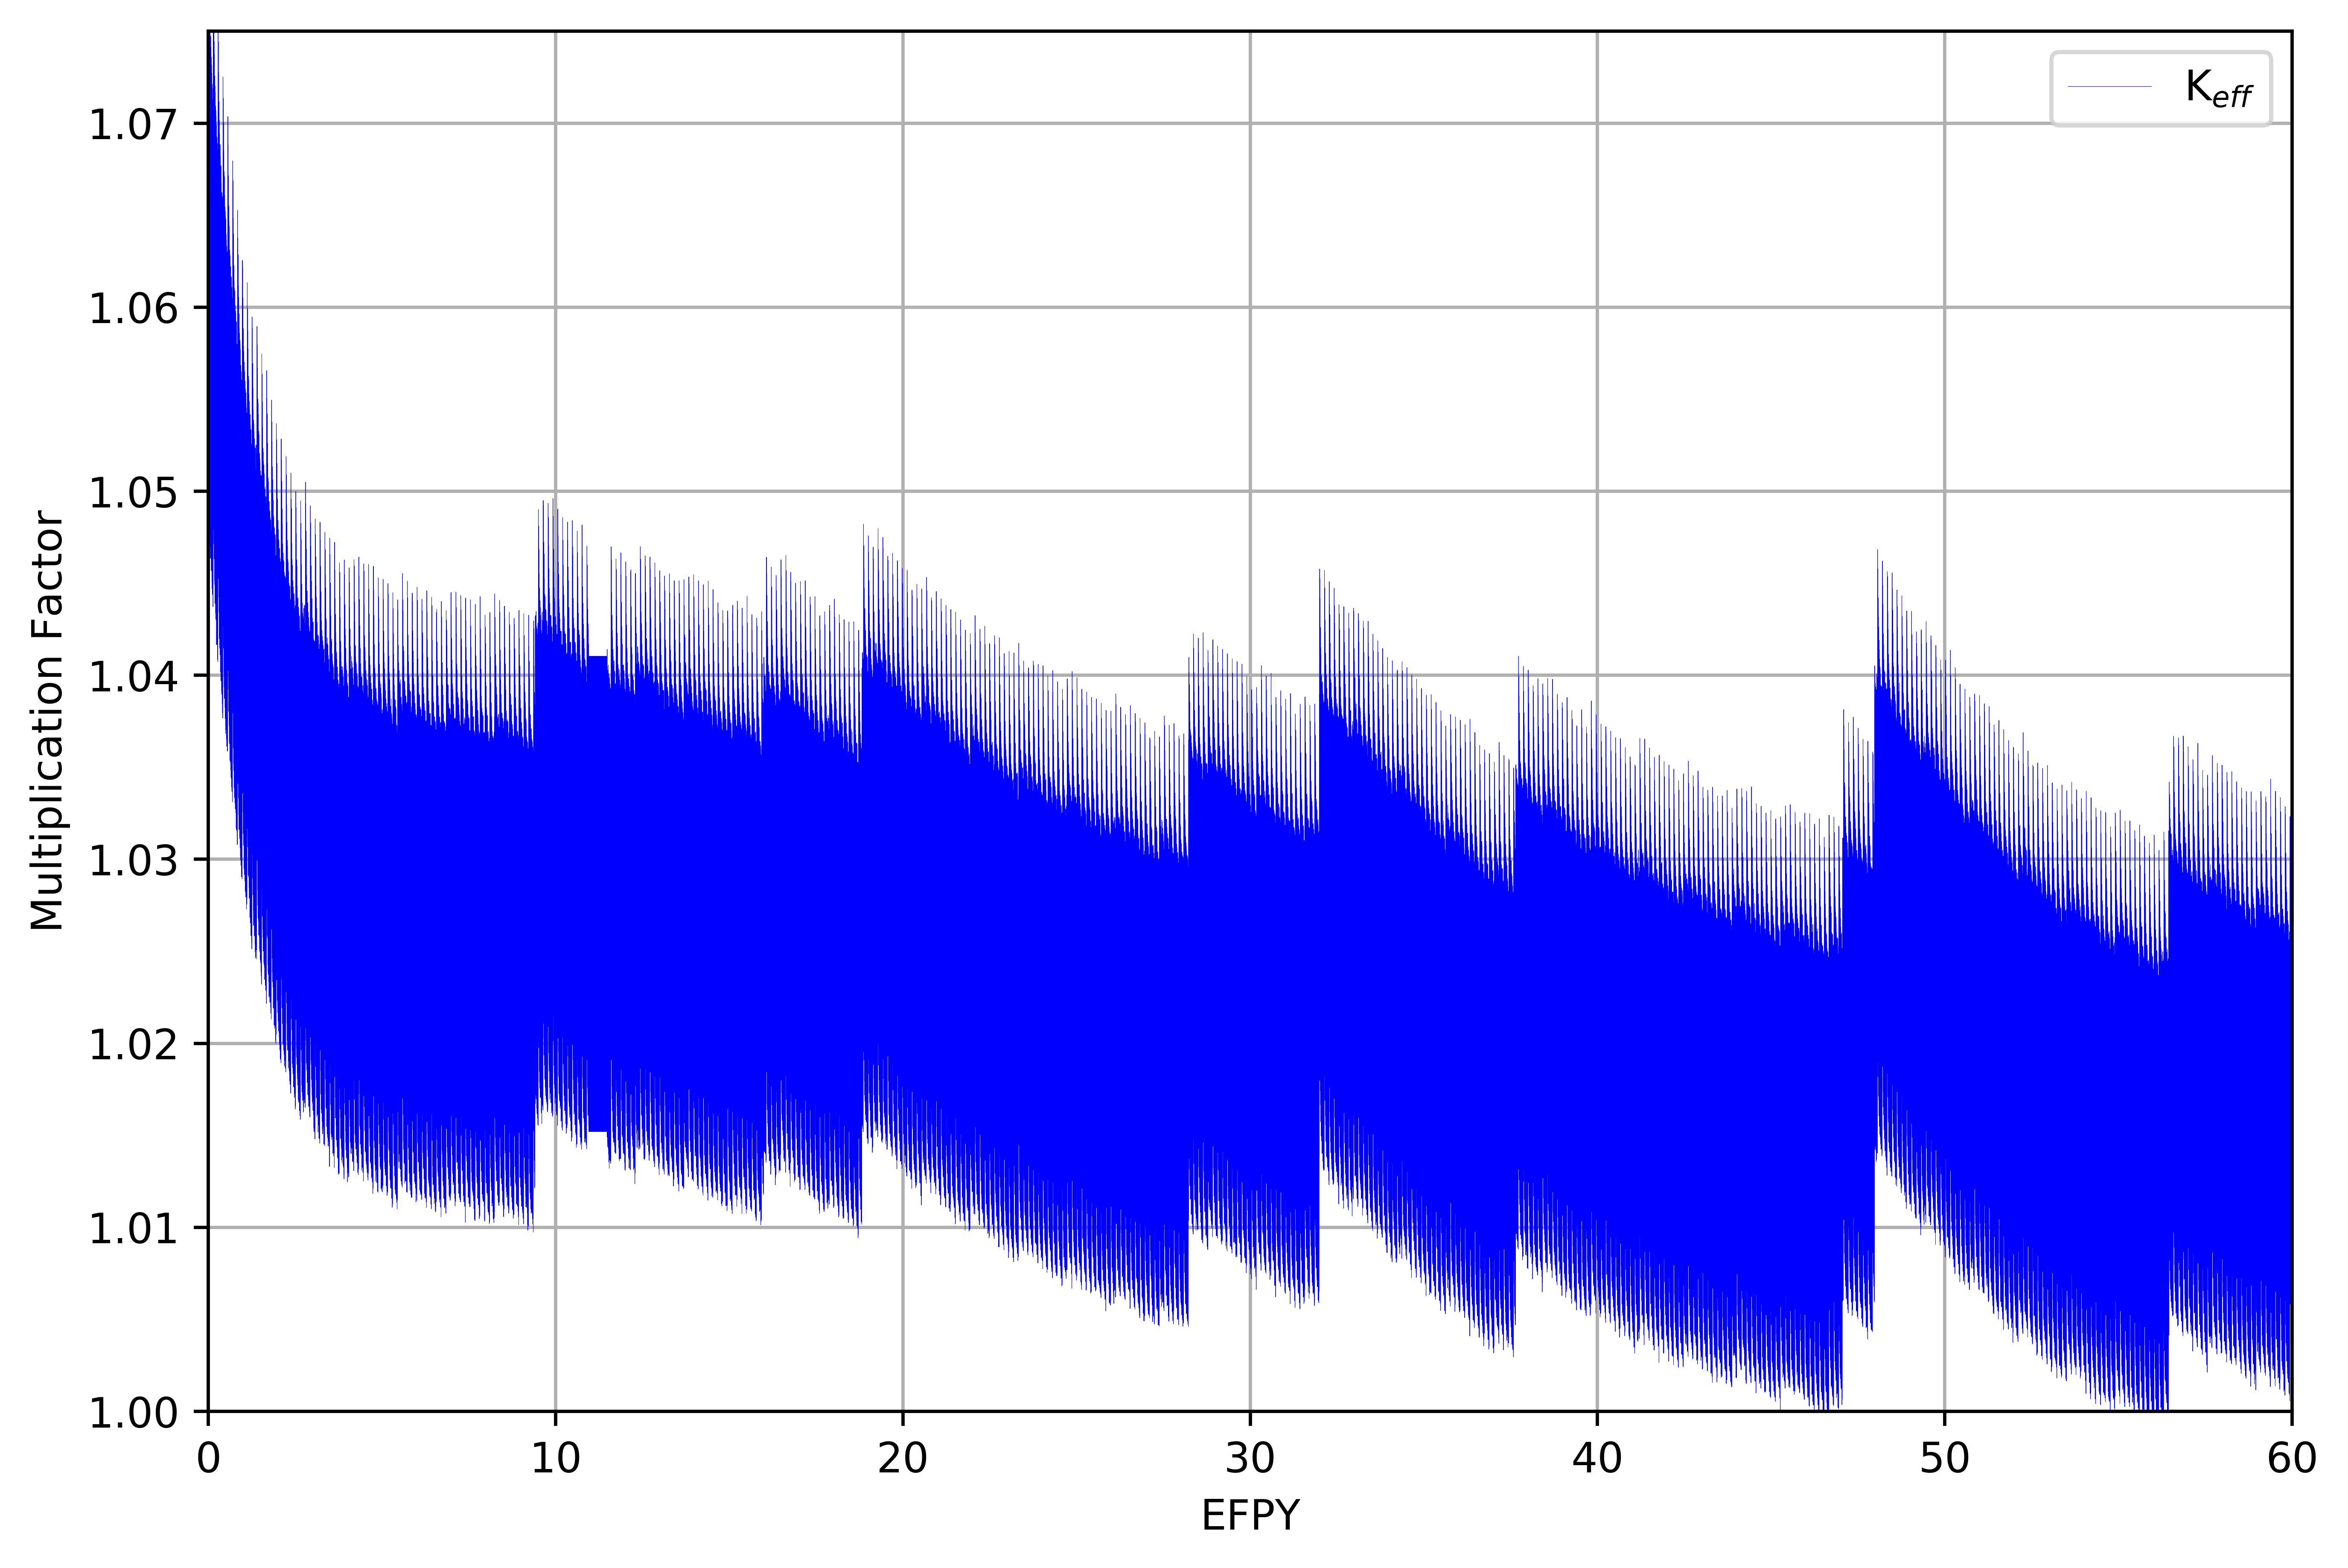
\includegraphics[width=\textwidth]{keff.png}
    \end{center}
	\caption{Effective multiplication factor dynamics for full-core model for a 60-year reactor operation. The confidence interval $\sigma=\pm15pcm$ is shaded.}
	\label{fig:keff}
\end{figure}
\begin{figure}[htbp!]
    \begin{center}
		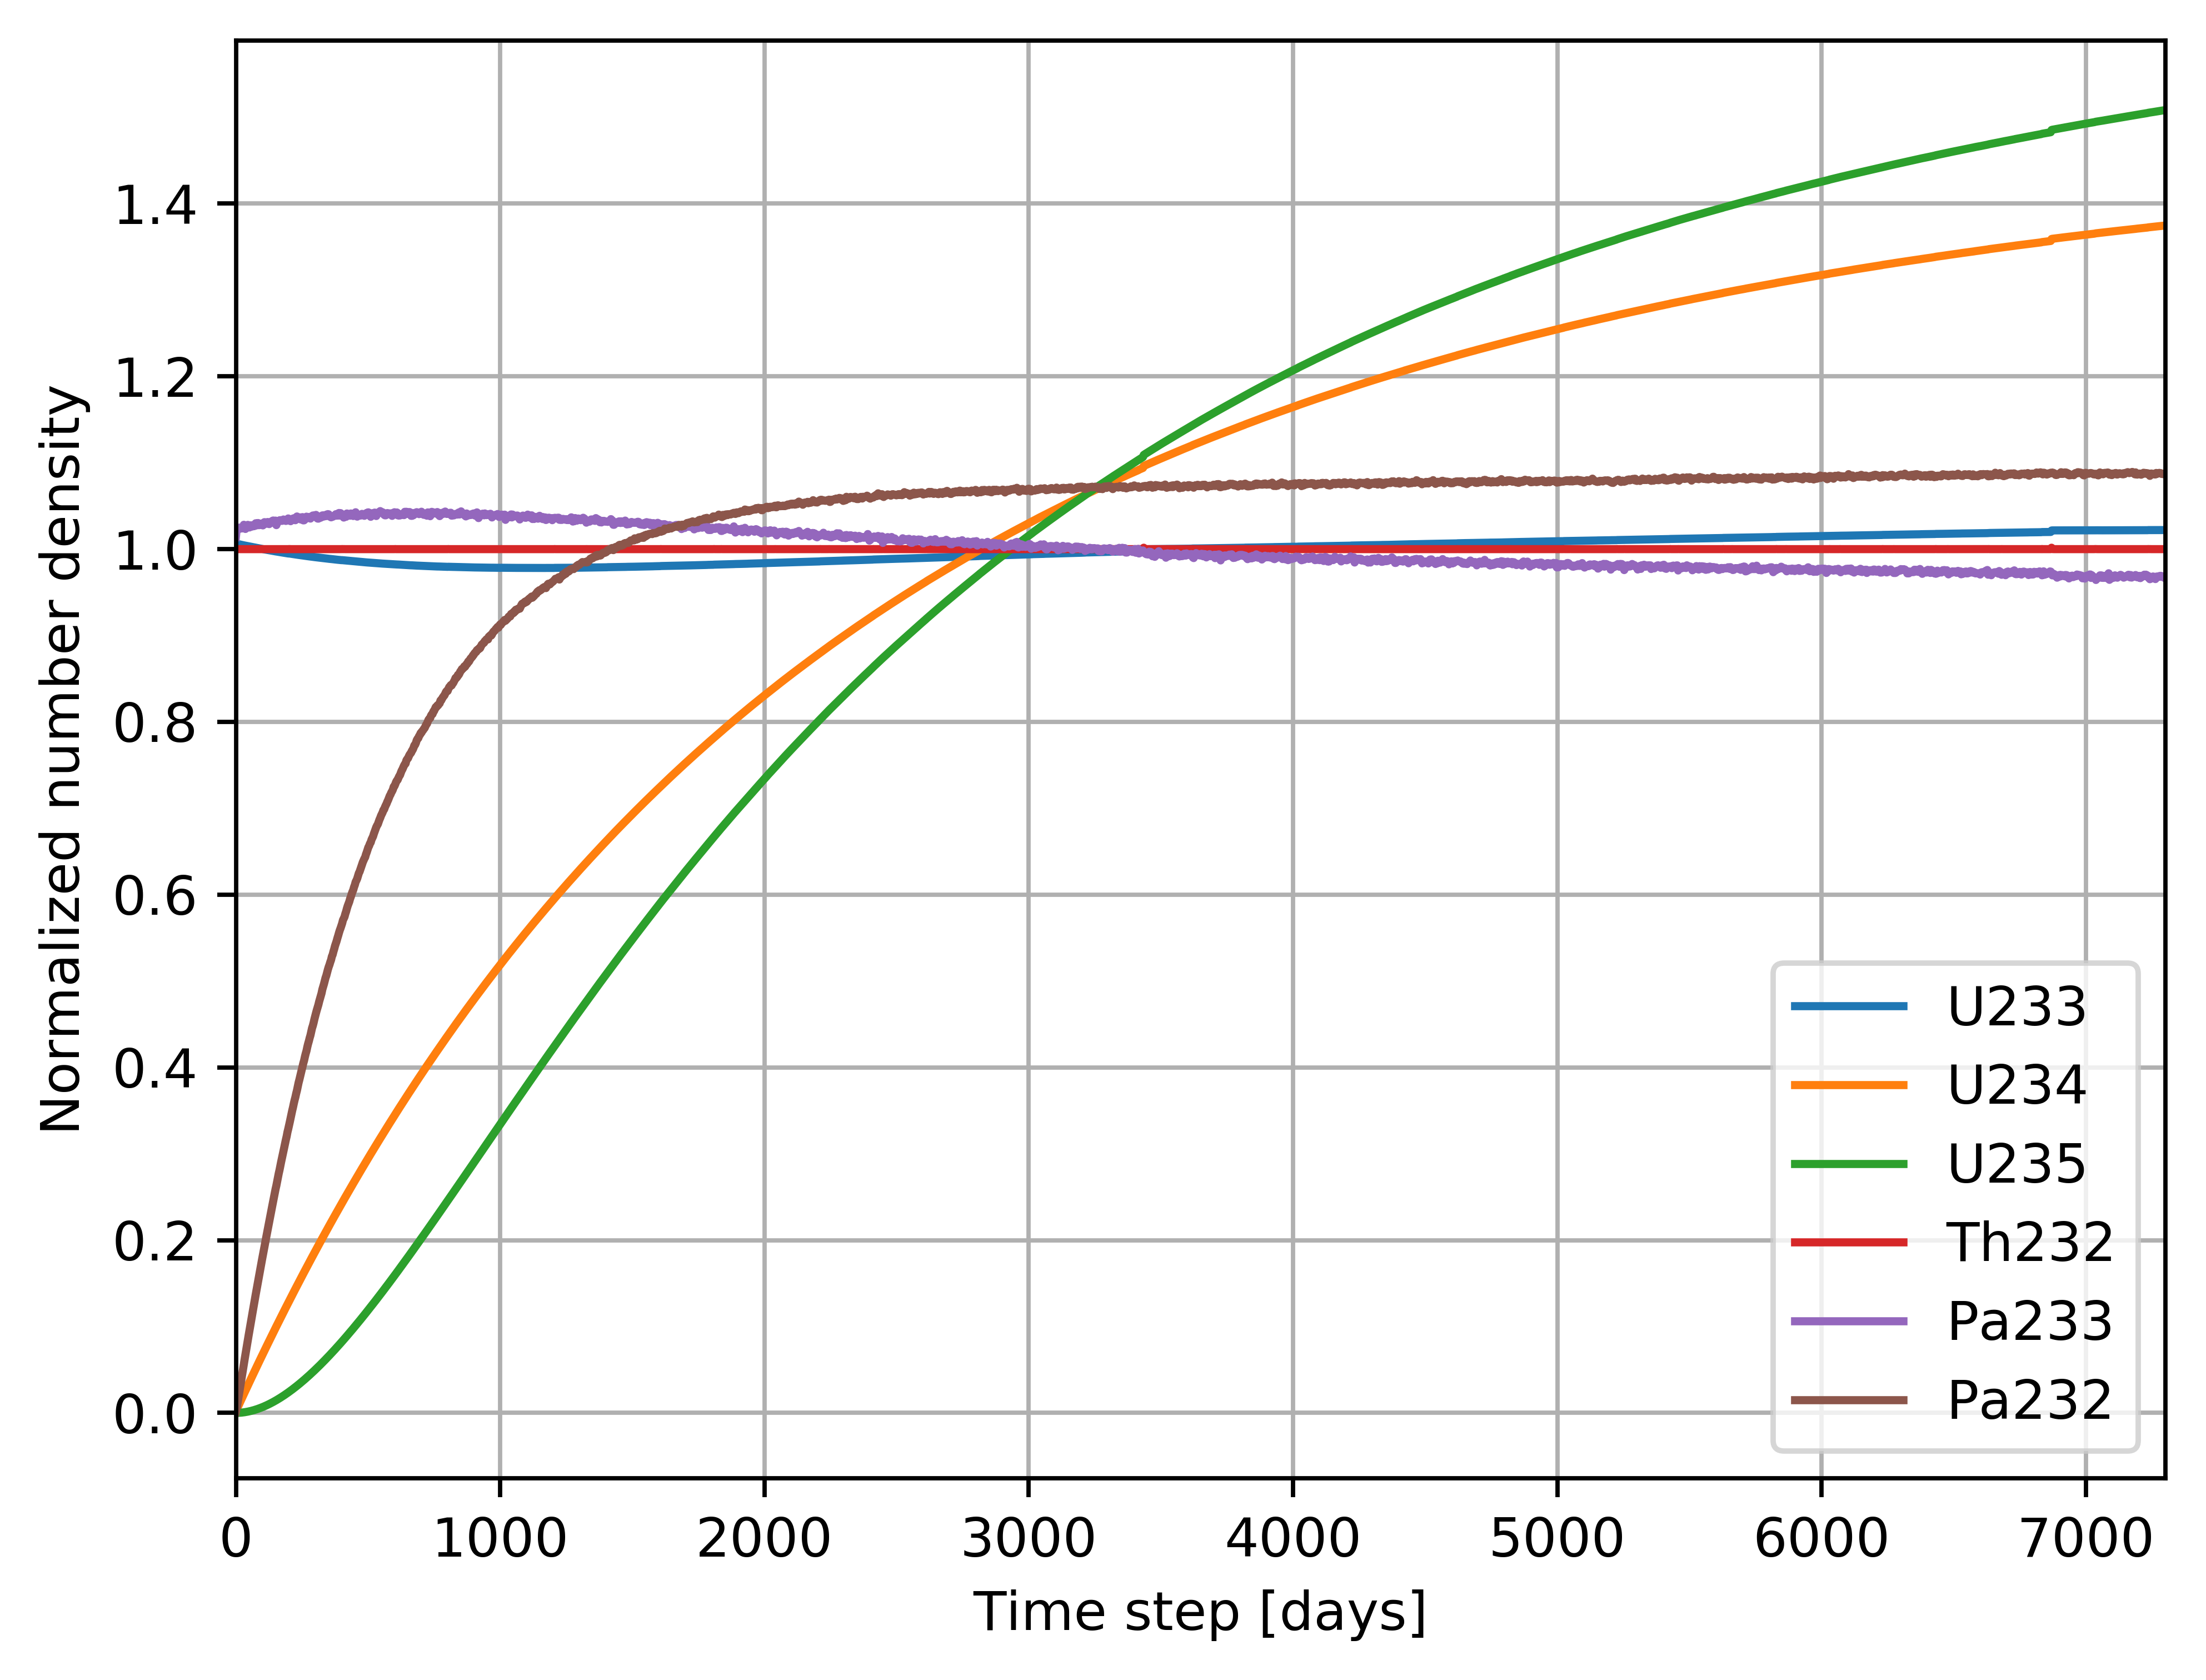
\includegraphics[width=\textwidth]{major_isotopes_adens.png}
    \end{center}
	\caption{Number density of major nuclides during 60 years of reactor operation.}
	\label{fig:adens_eq}
\end{figure}
\begin{figure}[htbp!]
    \begin{center}
		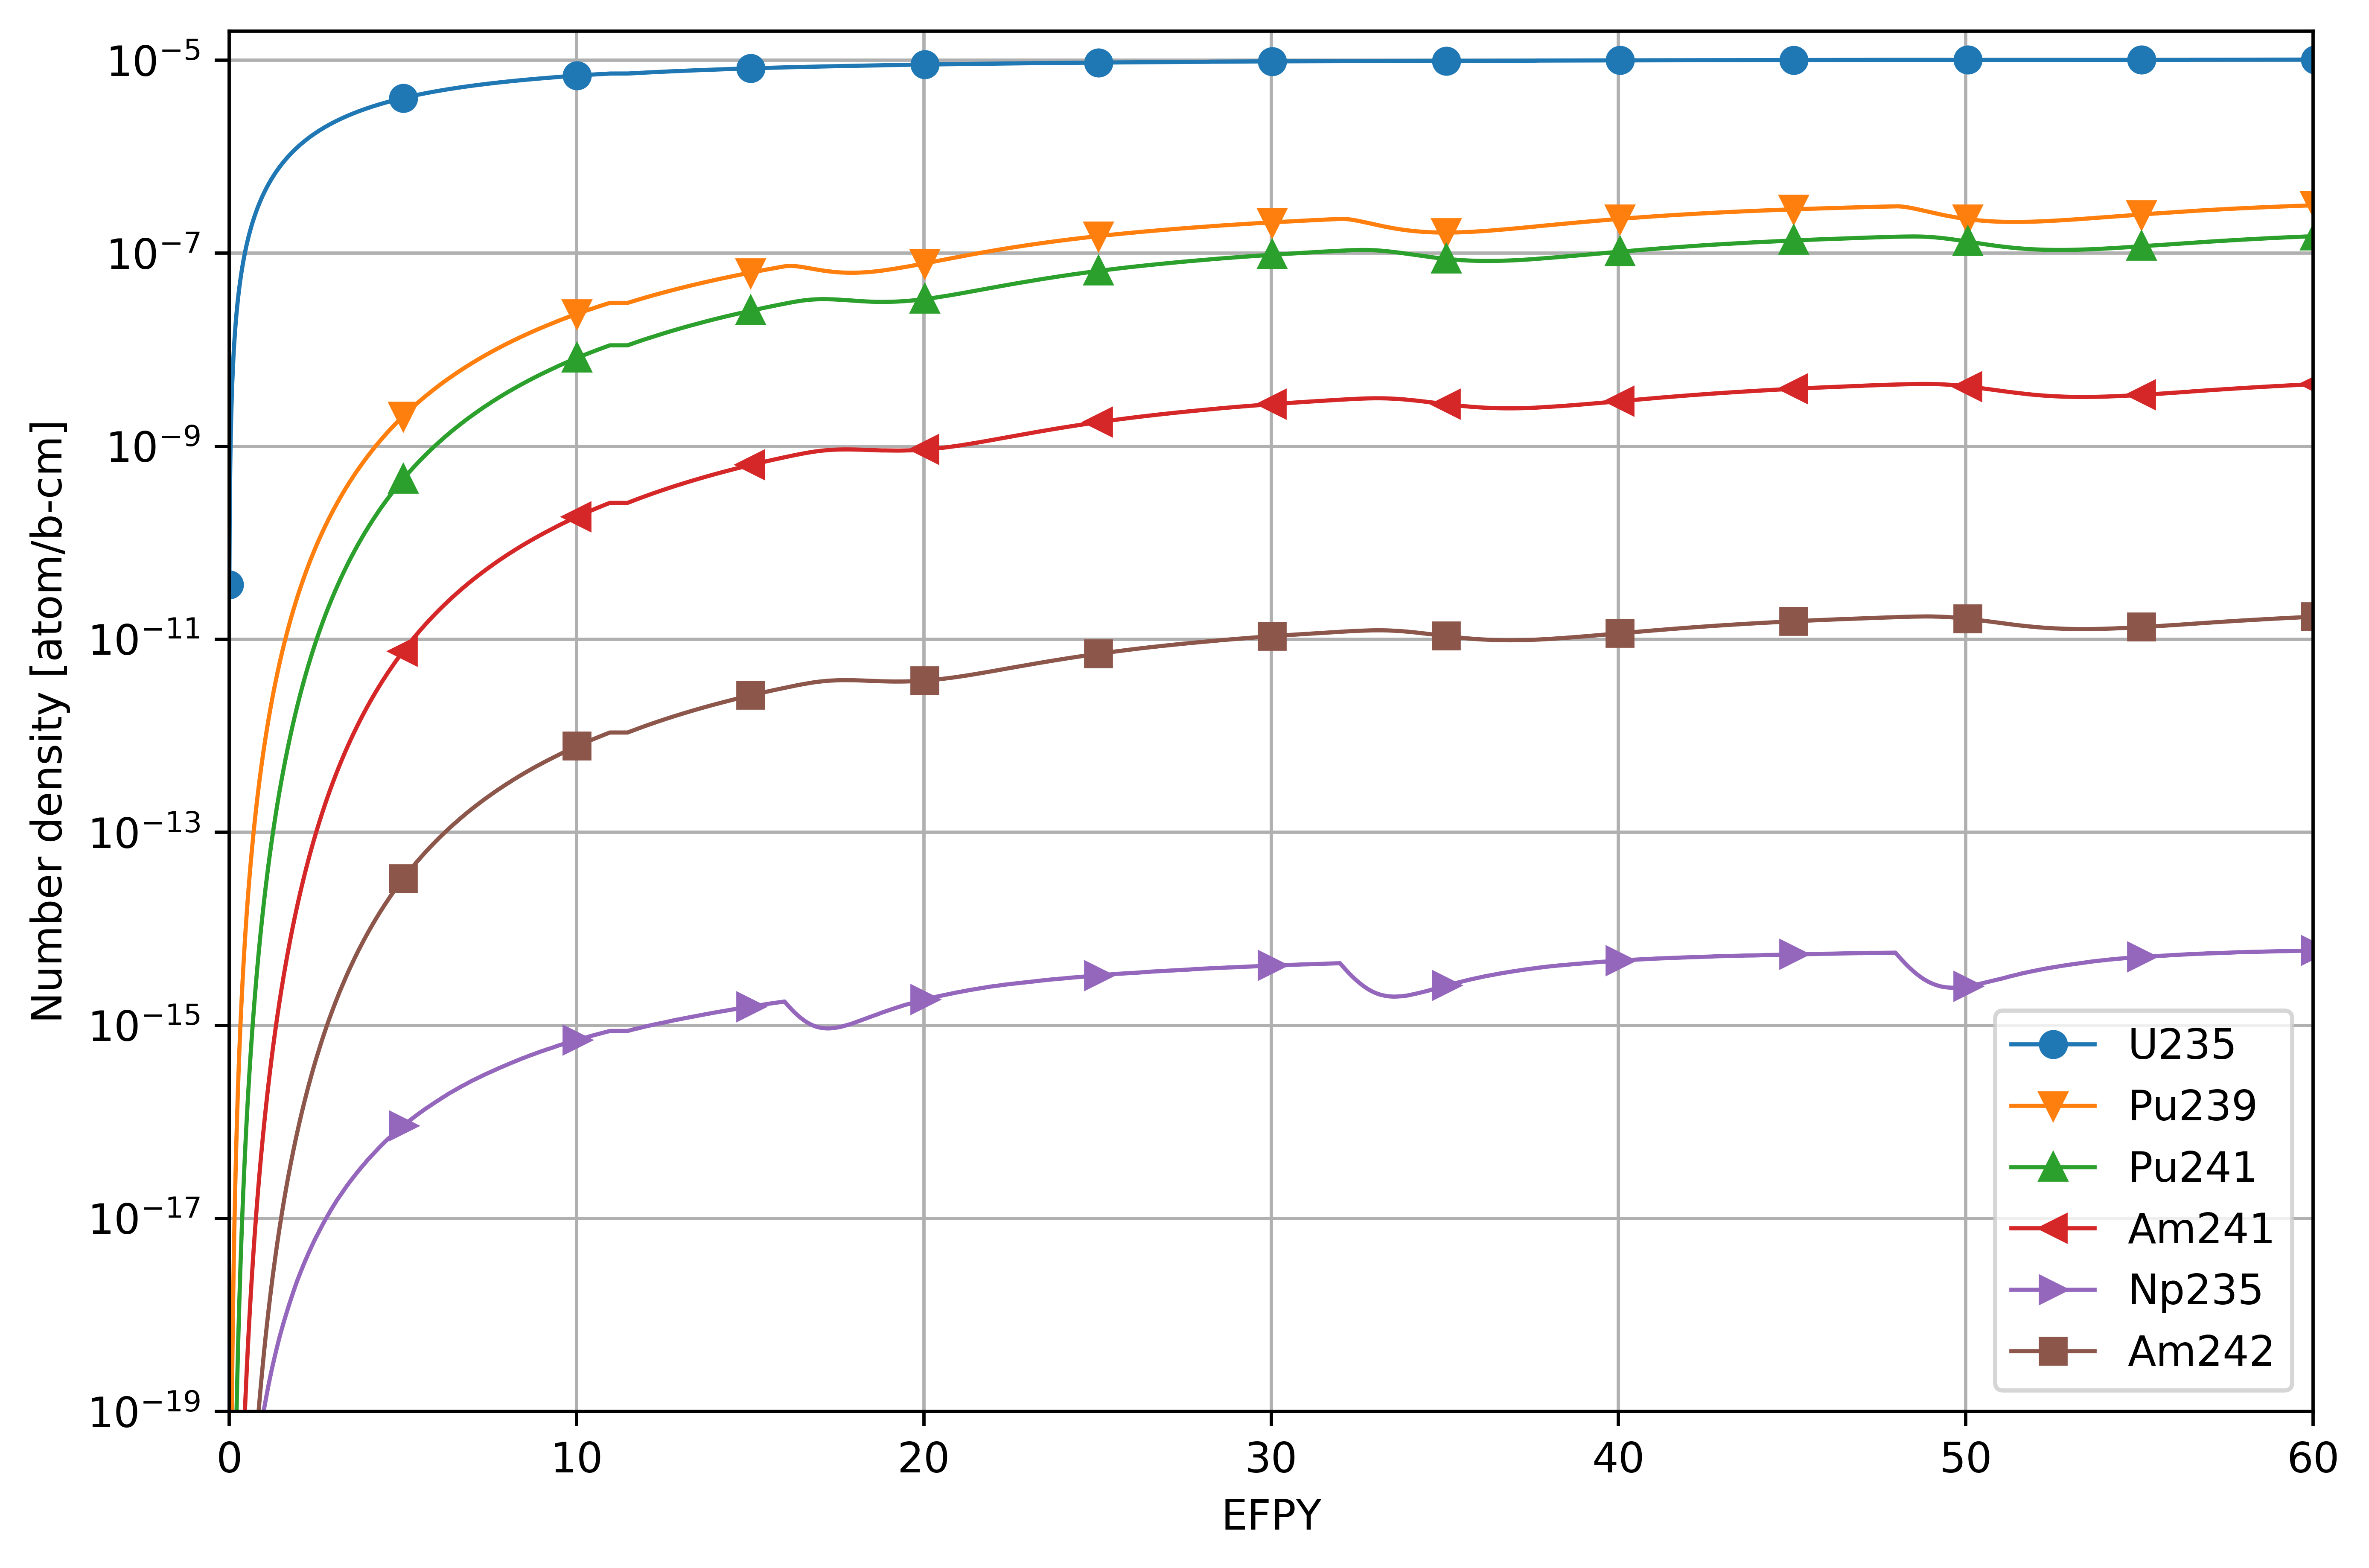
\includegraphics[width=\textwidth]{fissile_short.png}
    \end{center}
	\caption{Number density of fissile in epithermal spectrum nuclides accumulation during the reactor operation.}
	\label{fig:fissile_short}
\end{figure}
\begin{figure}[htbp!]
    \begin{center}
		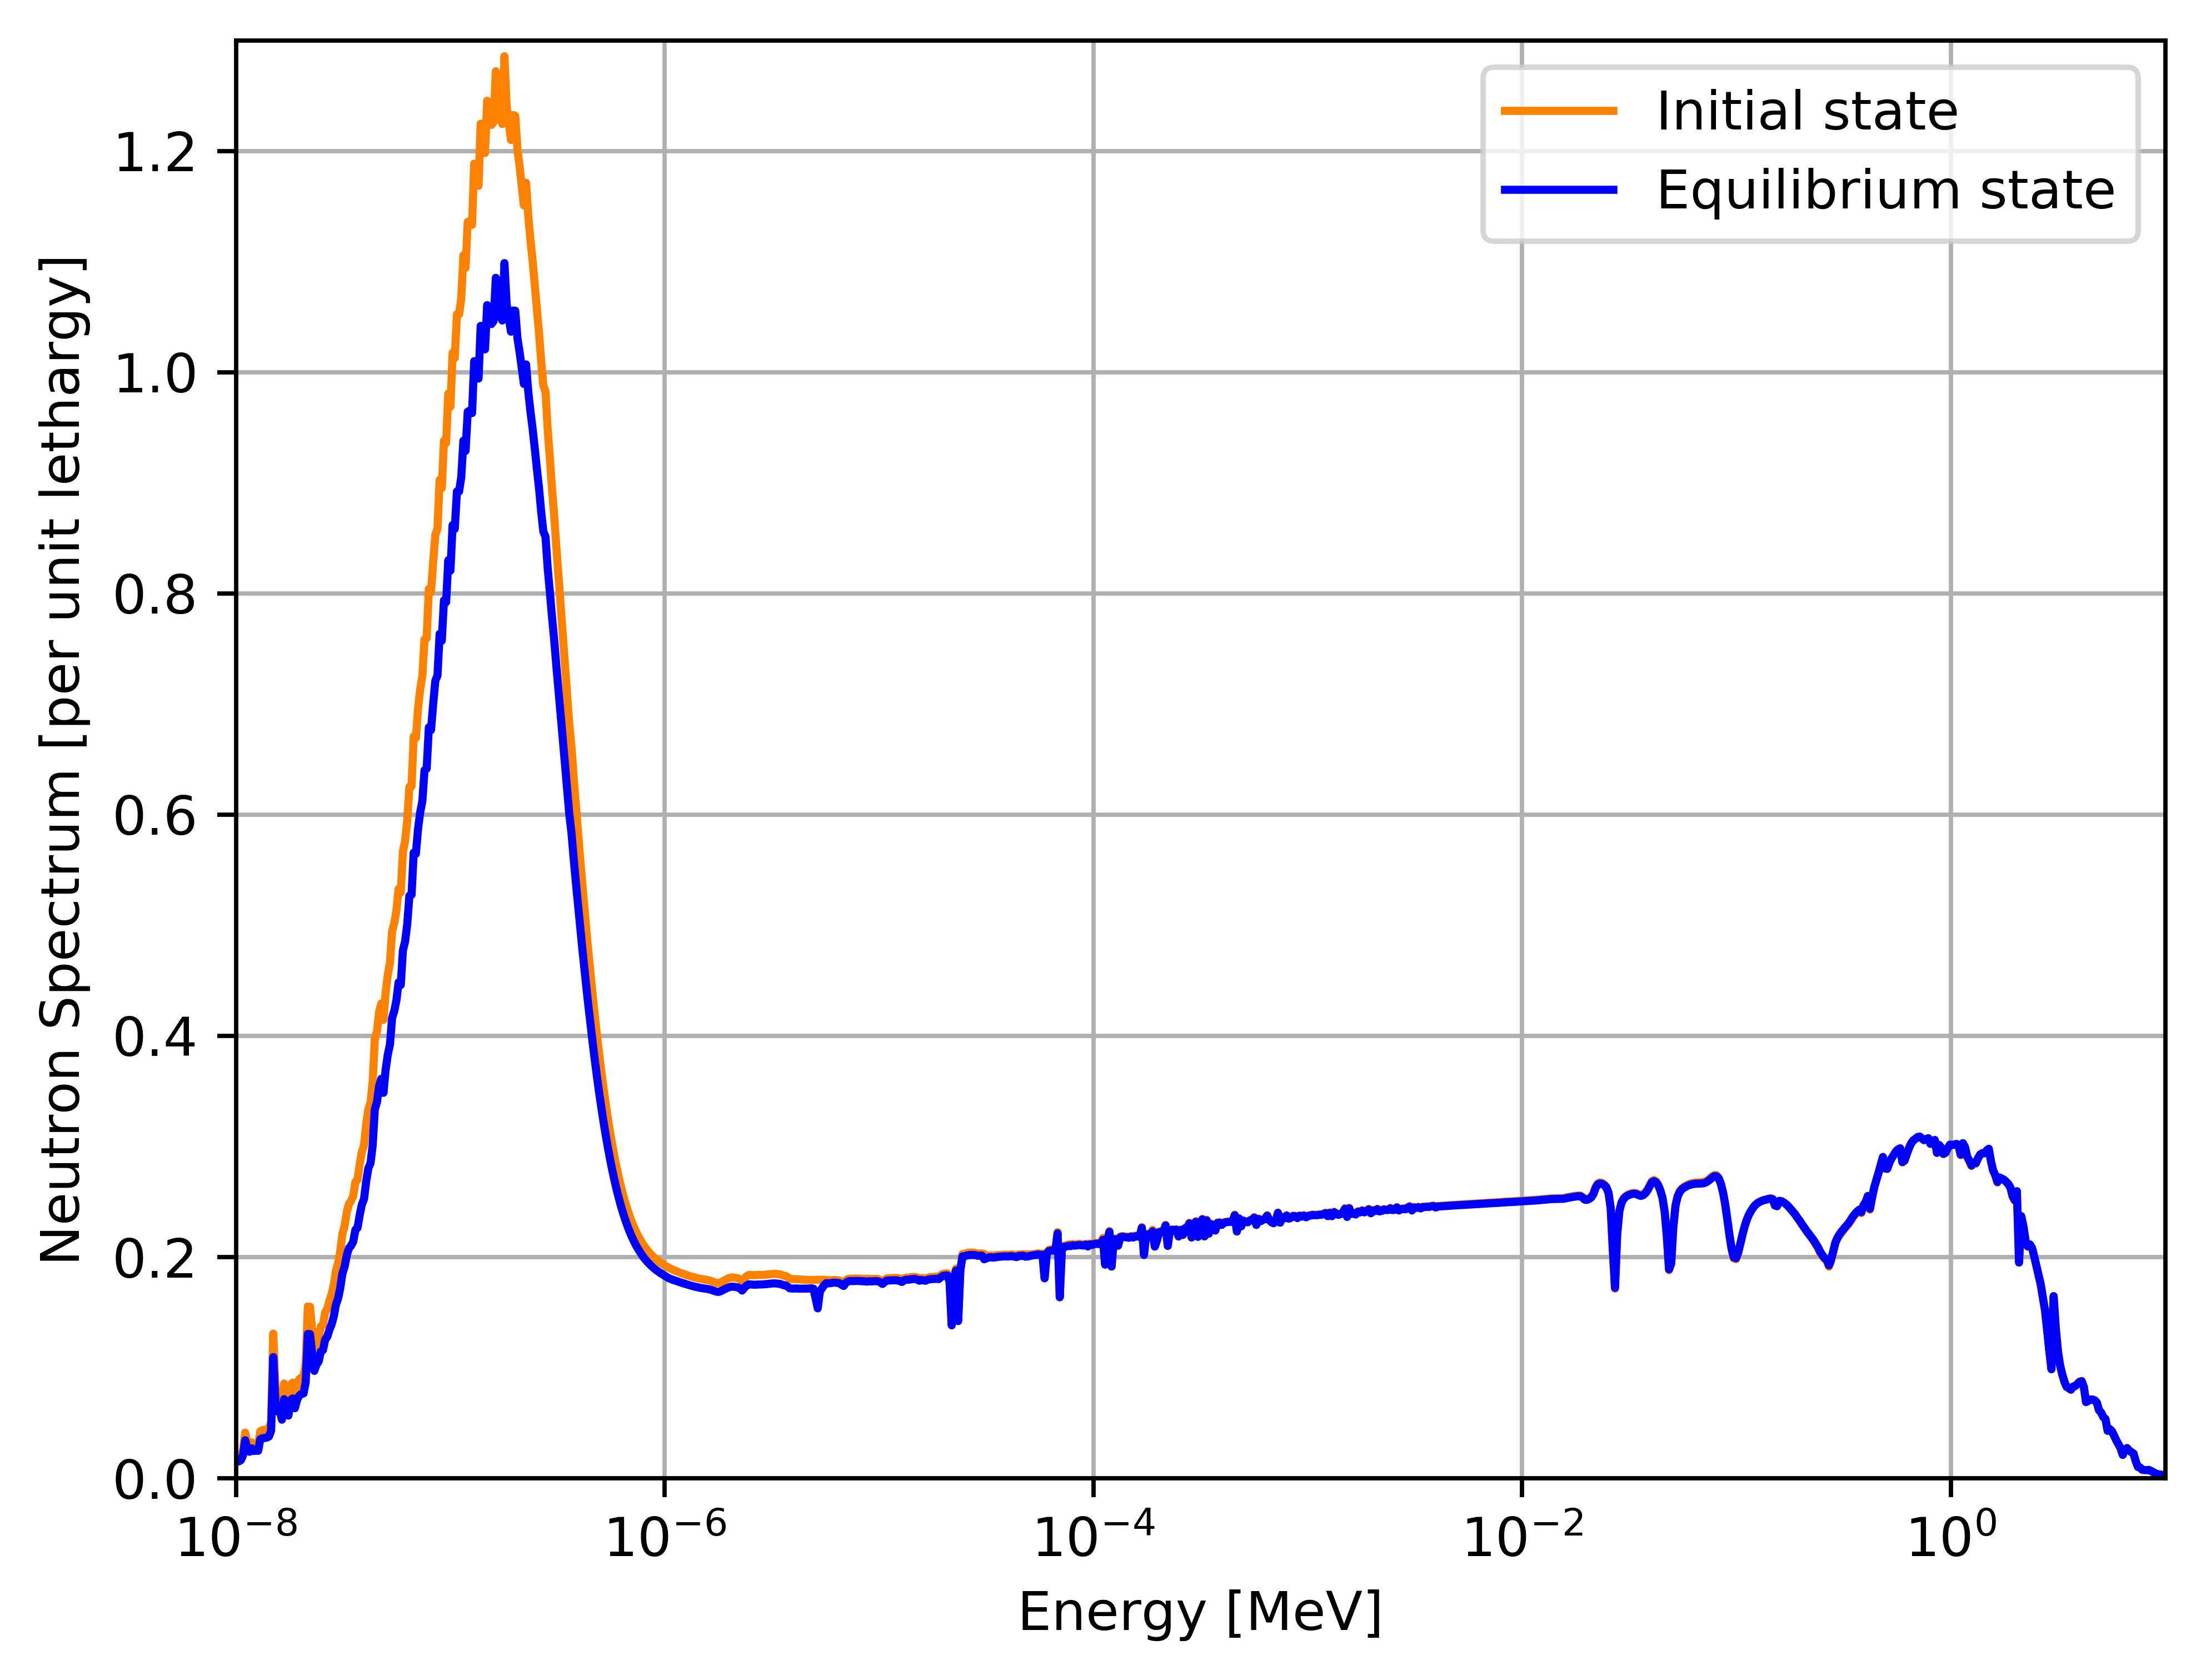
\includegraphics[width=\textwidth]{spectrum.png} 
    \end{center}
	\caption{Neutron flux energy spectrum normalized by unit lethargy for initial and equilibrium fuel salt composition.}
	\label{fig:spectrum}
\end{figure}
\begin{figure}[htbp!]
    \begin{center}
		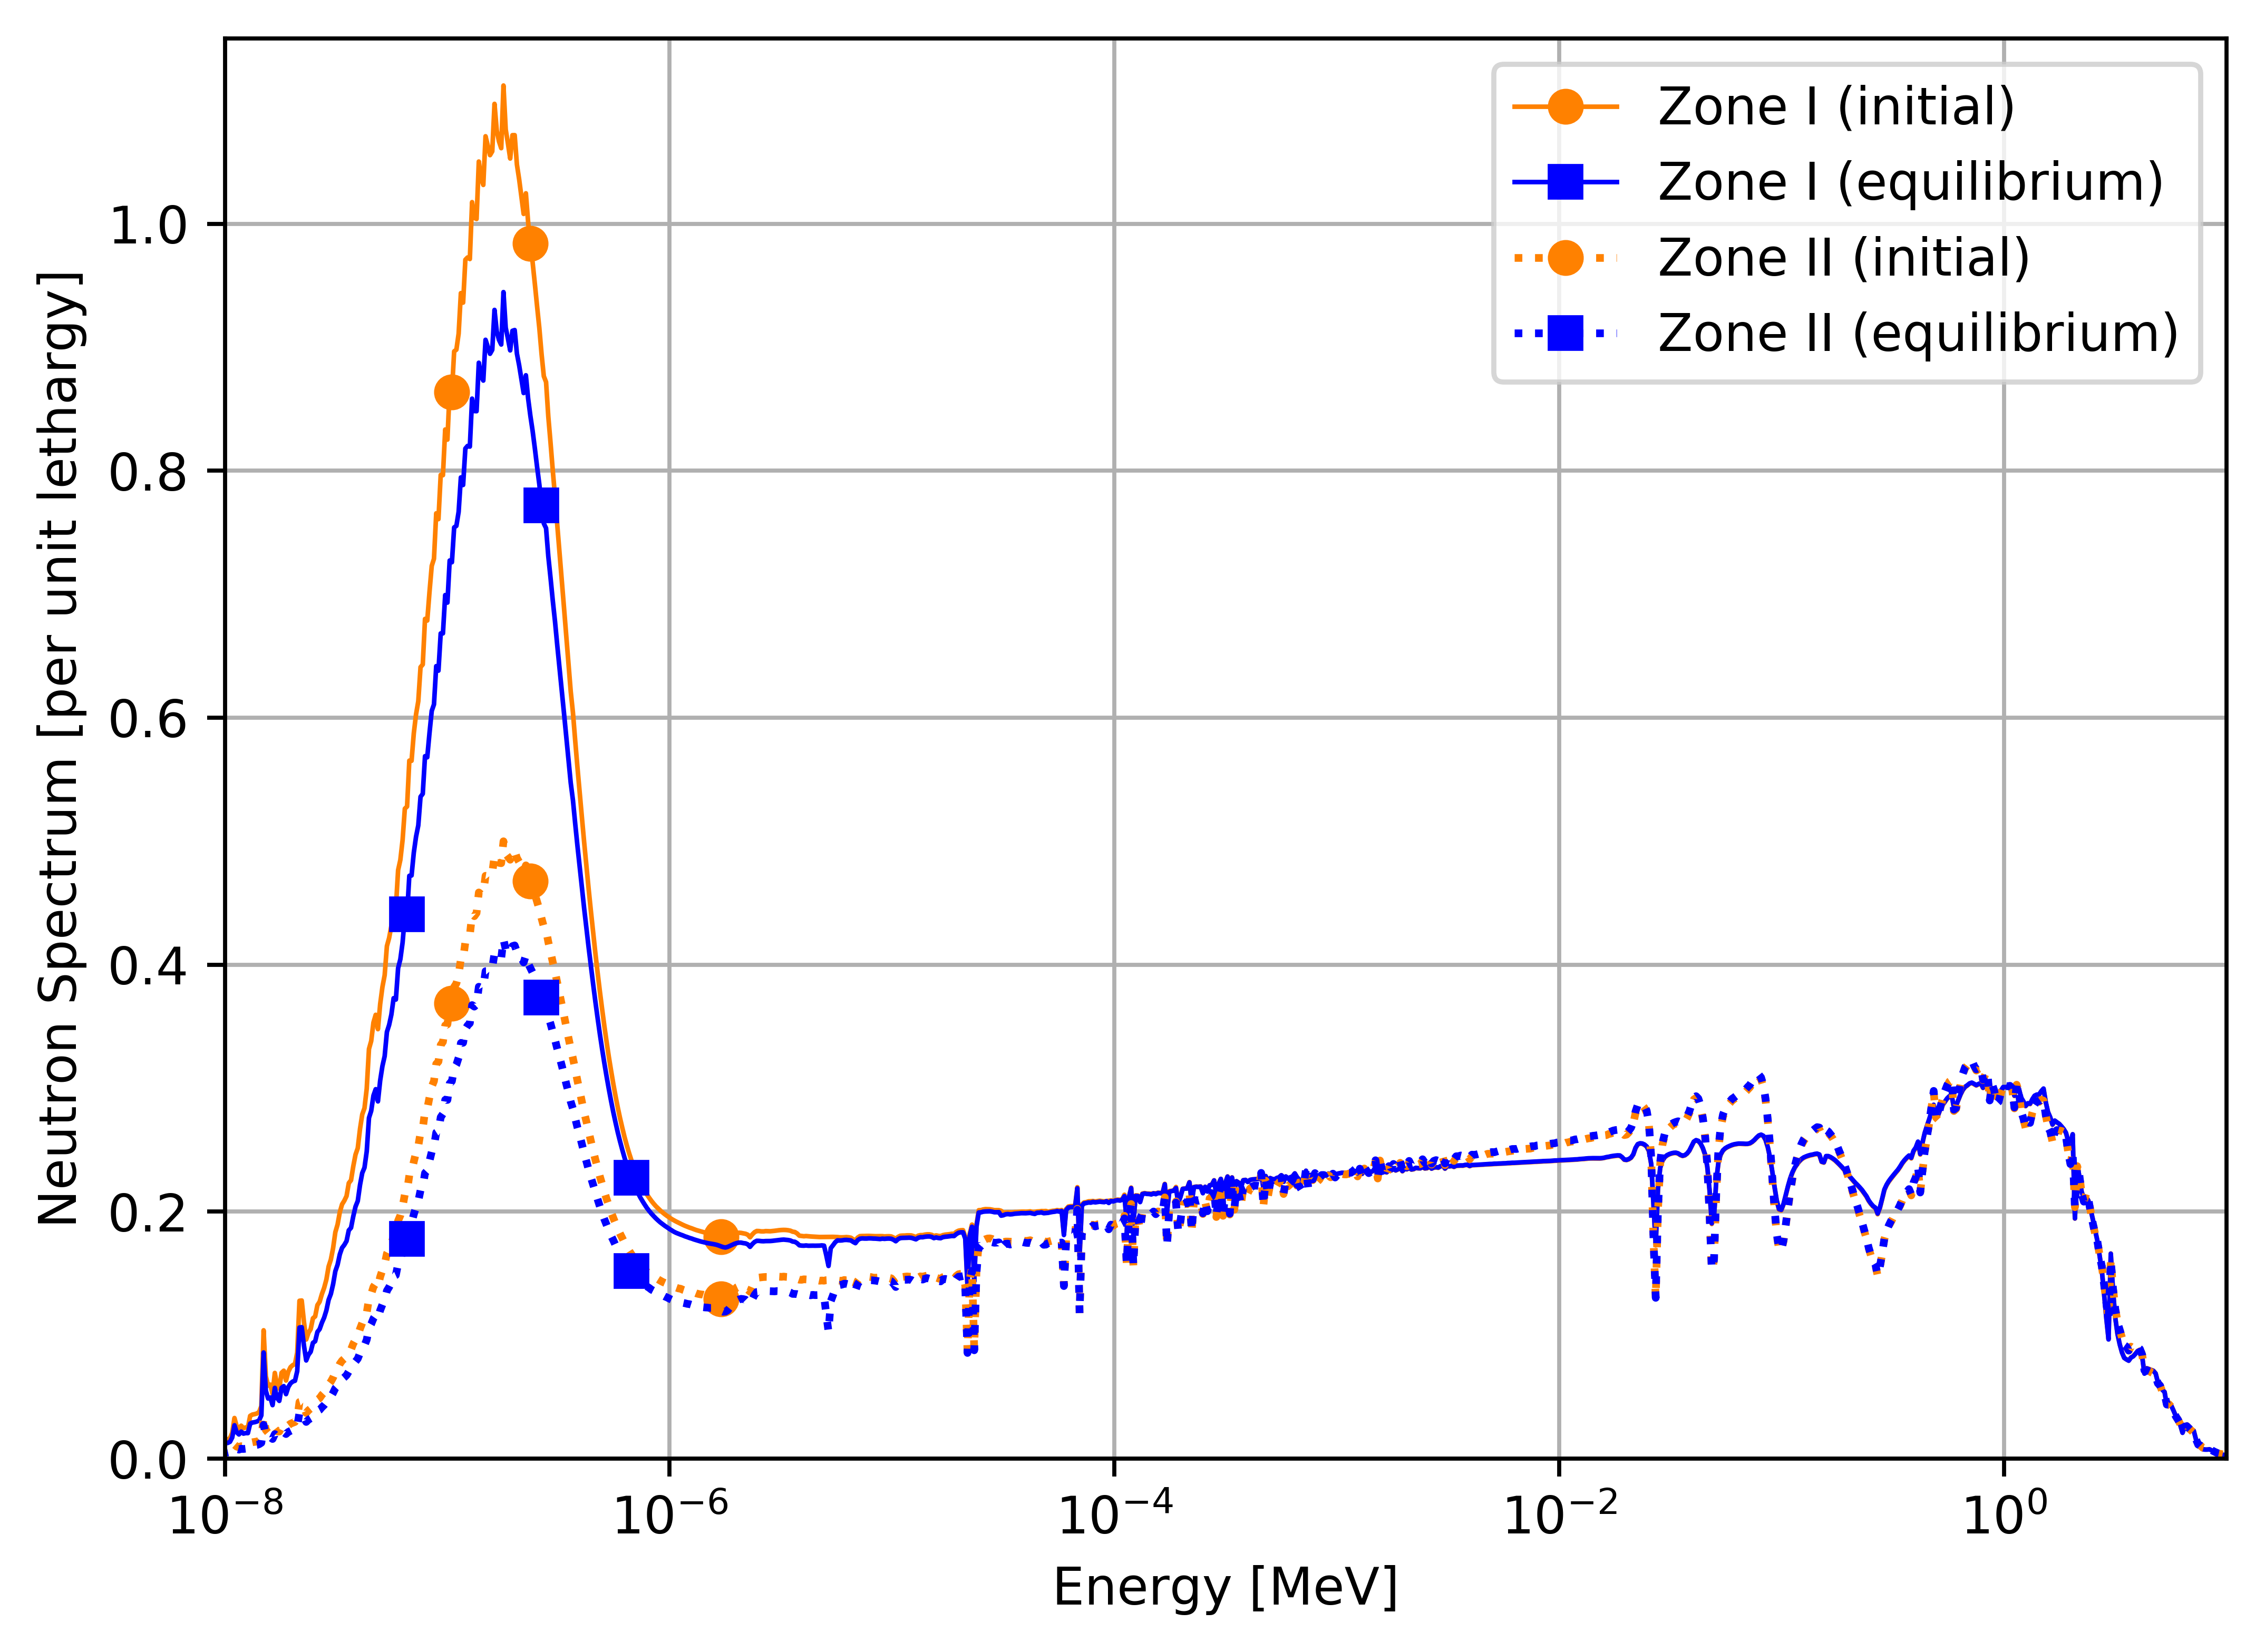
\includegraphics[width=\textwidth]{spectrum_zones.png} 
    \end{center}
	\caption{Neutron flux energy spectrum in different core regions normalized by unit lethargy for the initial and equilibrium fuel salt composition.}
	\label{fig:spectrum_zones}
\end{figure}
\begin{figure}[htbp!]
    \begin{center}
		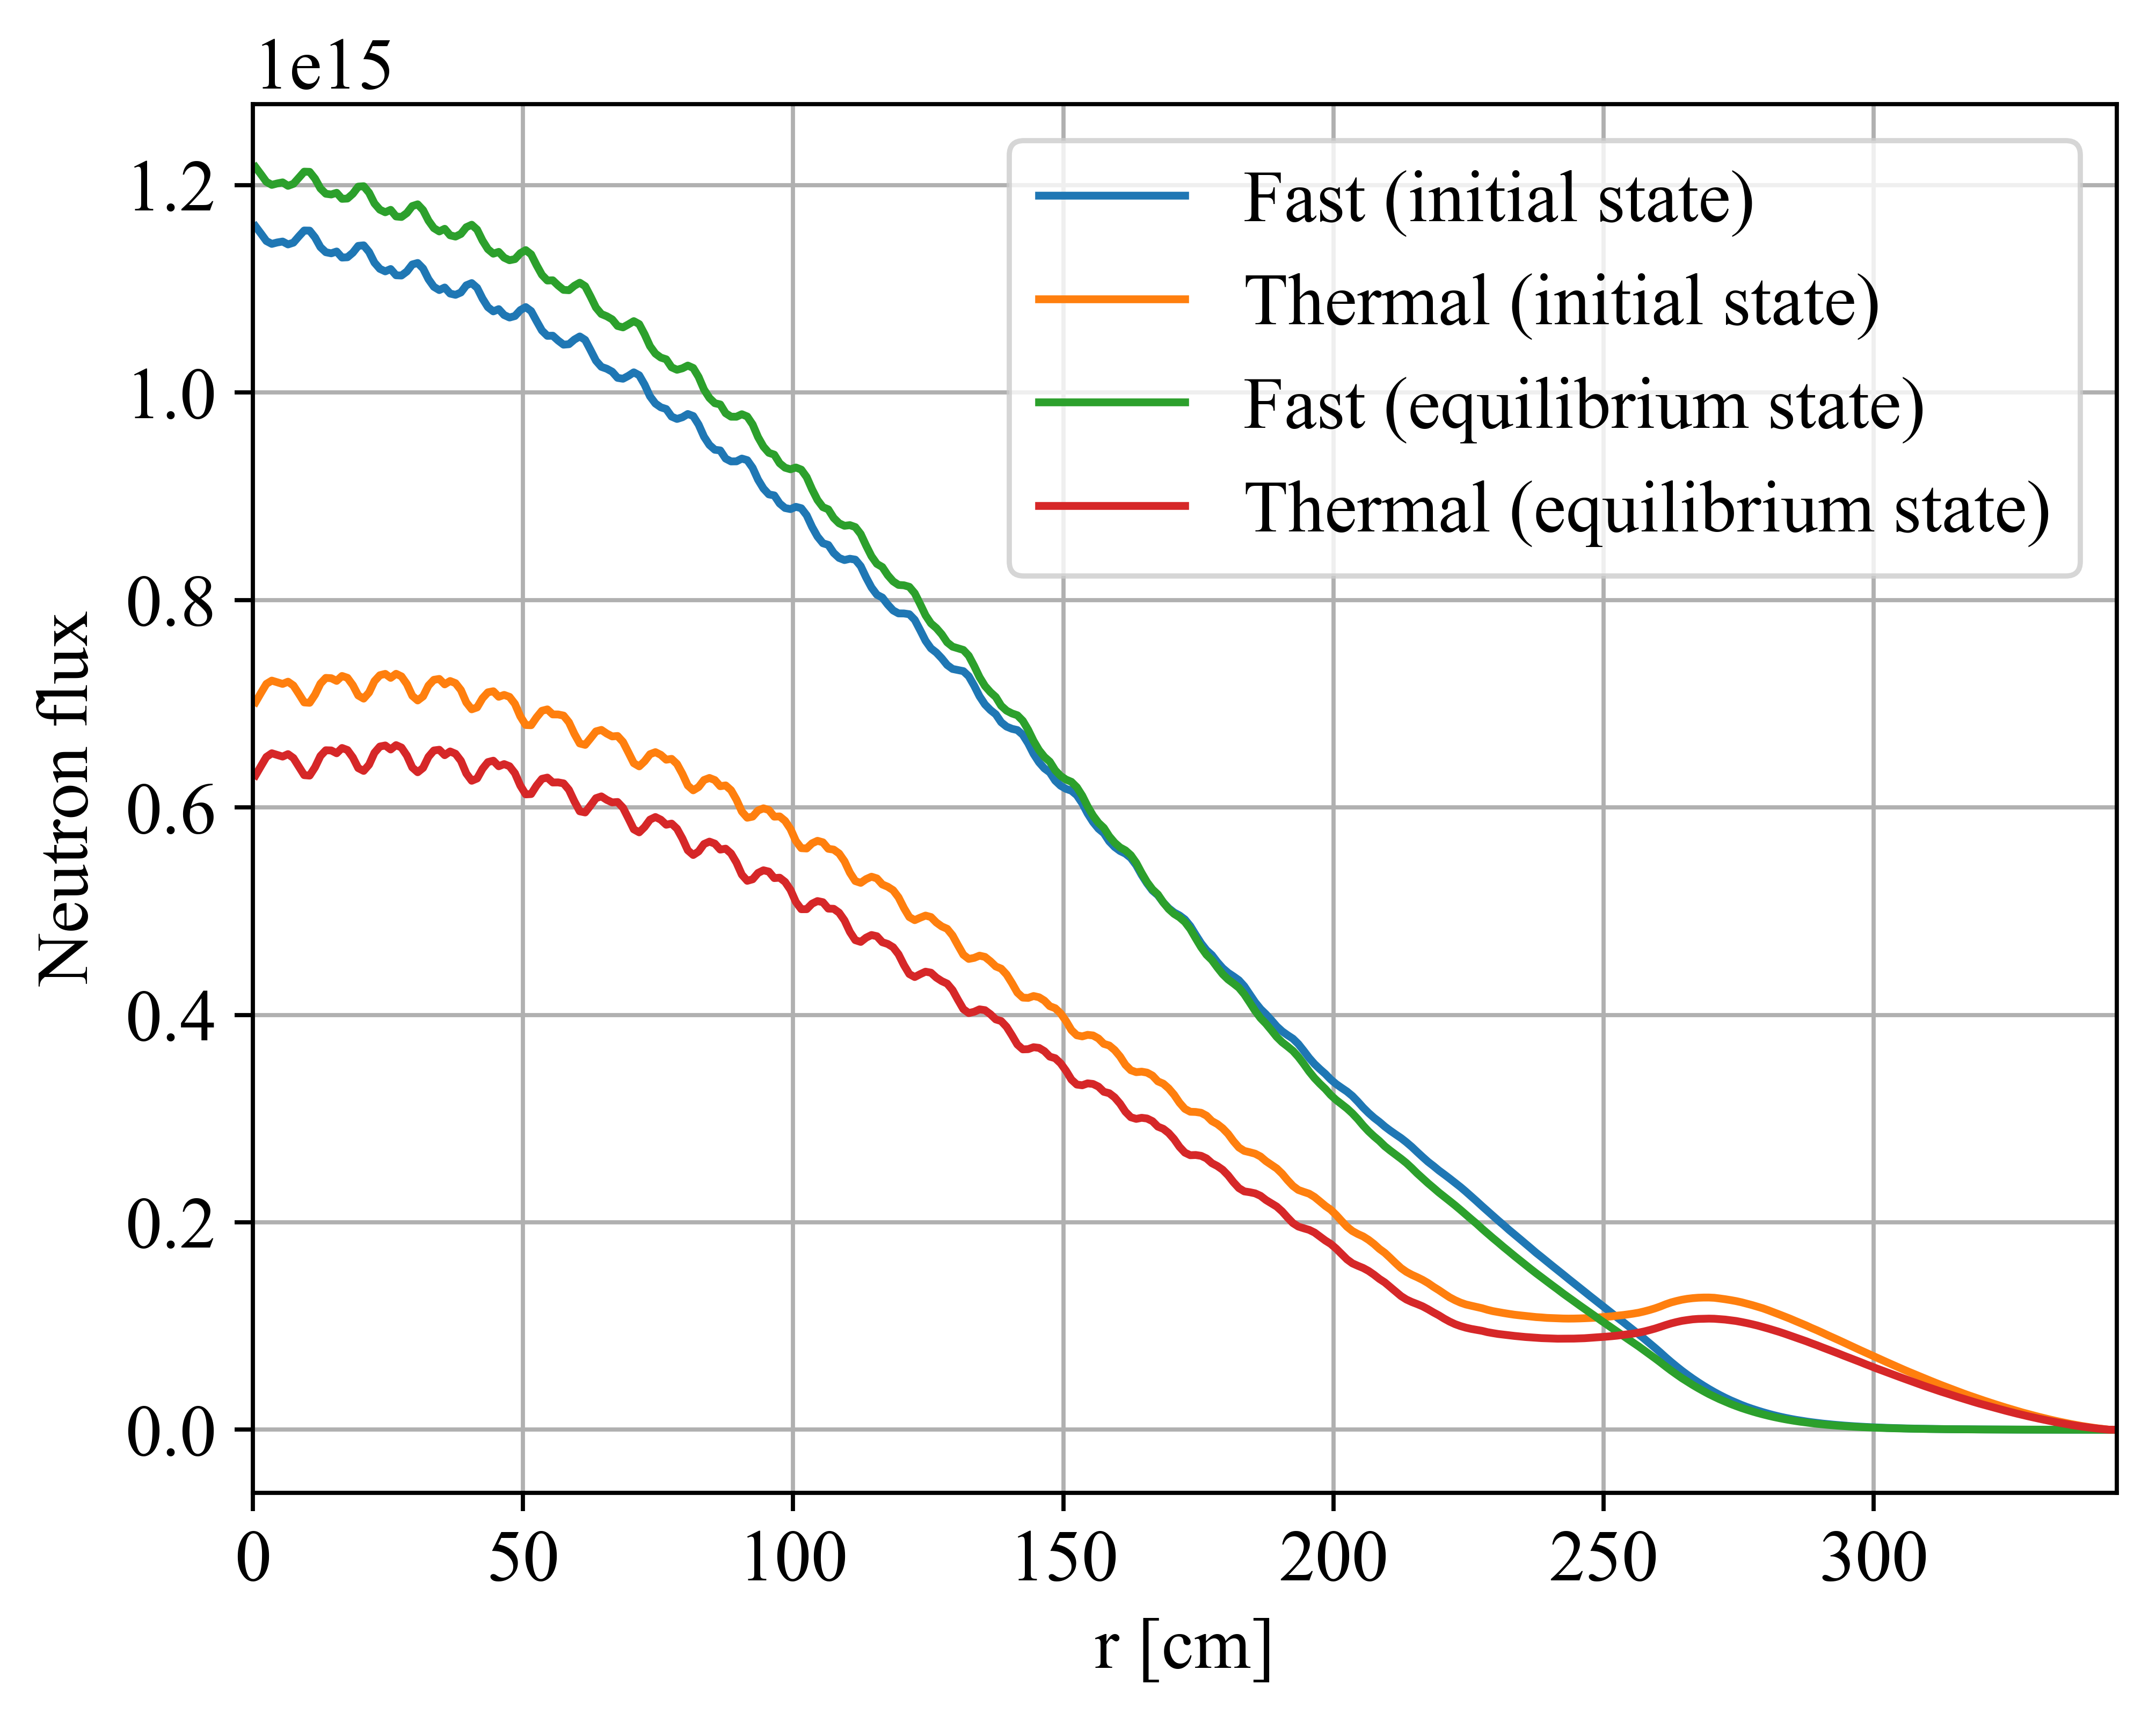
\includegraphics[width=\textwidth]{radial_flux.png} 
    \end{center}
	\caption{Radial neutron flux distribution for initial and equilibrium fuel salt composition.}
	\label{fig:radial_flux}
\end{figure}
\begin{figure}[htbp!]
    \begin{center}
		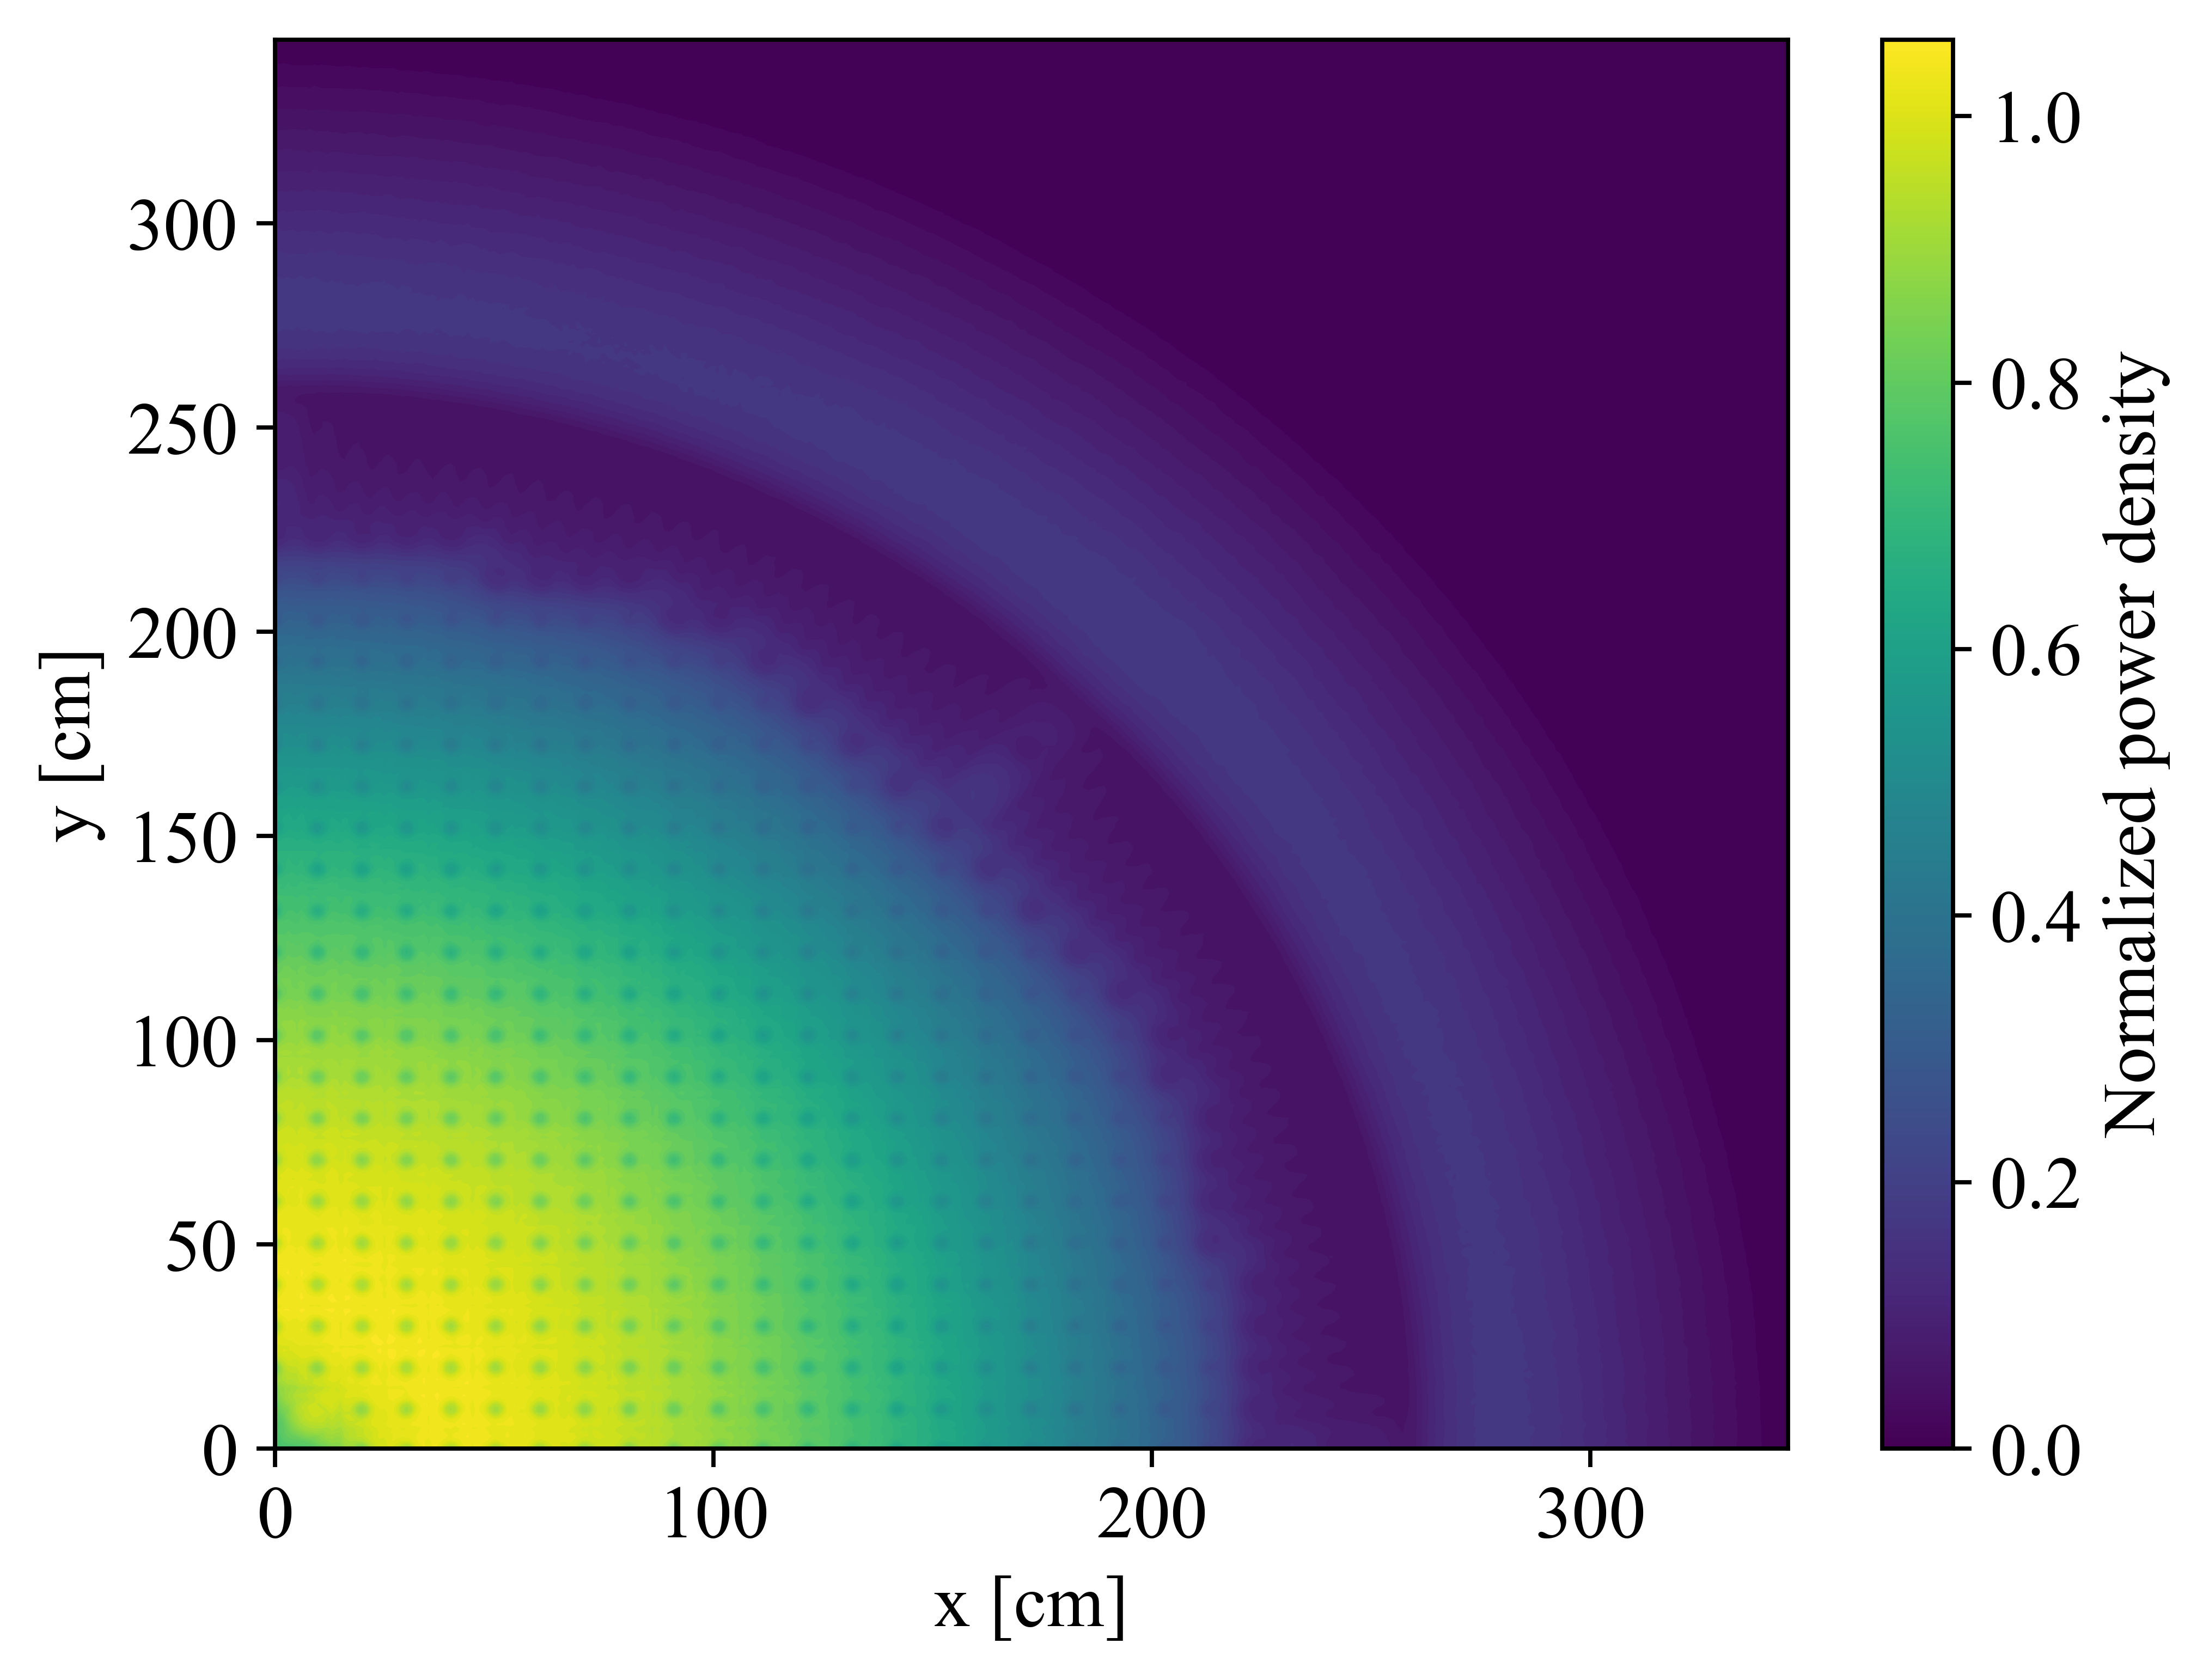
\includegraphics[width=\textwidth]{power_distribution_eq.png} 
    \end{center}
	\caption{Normalized power density for both initial and equilibrium fuel salt composition.}
	\label{fig:pow_den}
\end{figure}
\begin{figure}[htbp!]
    \begin{center}
		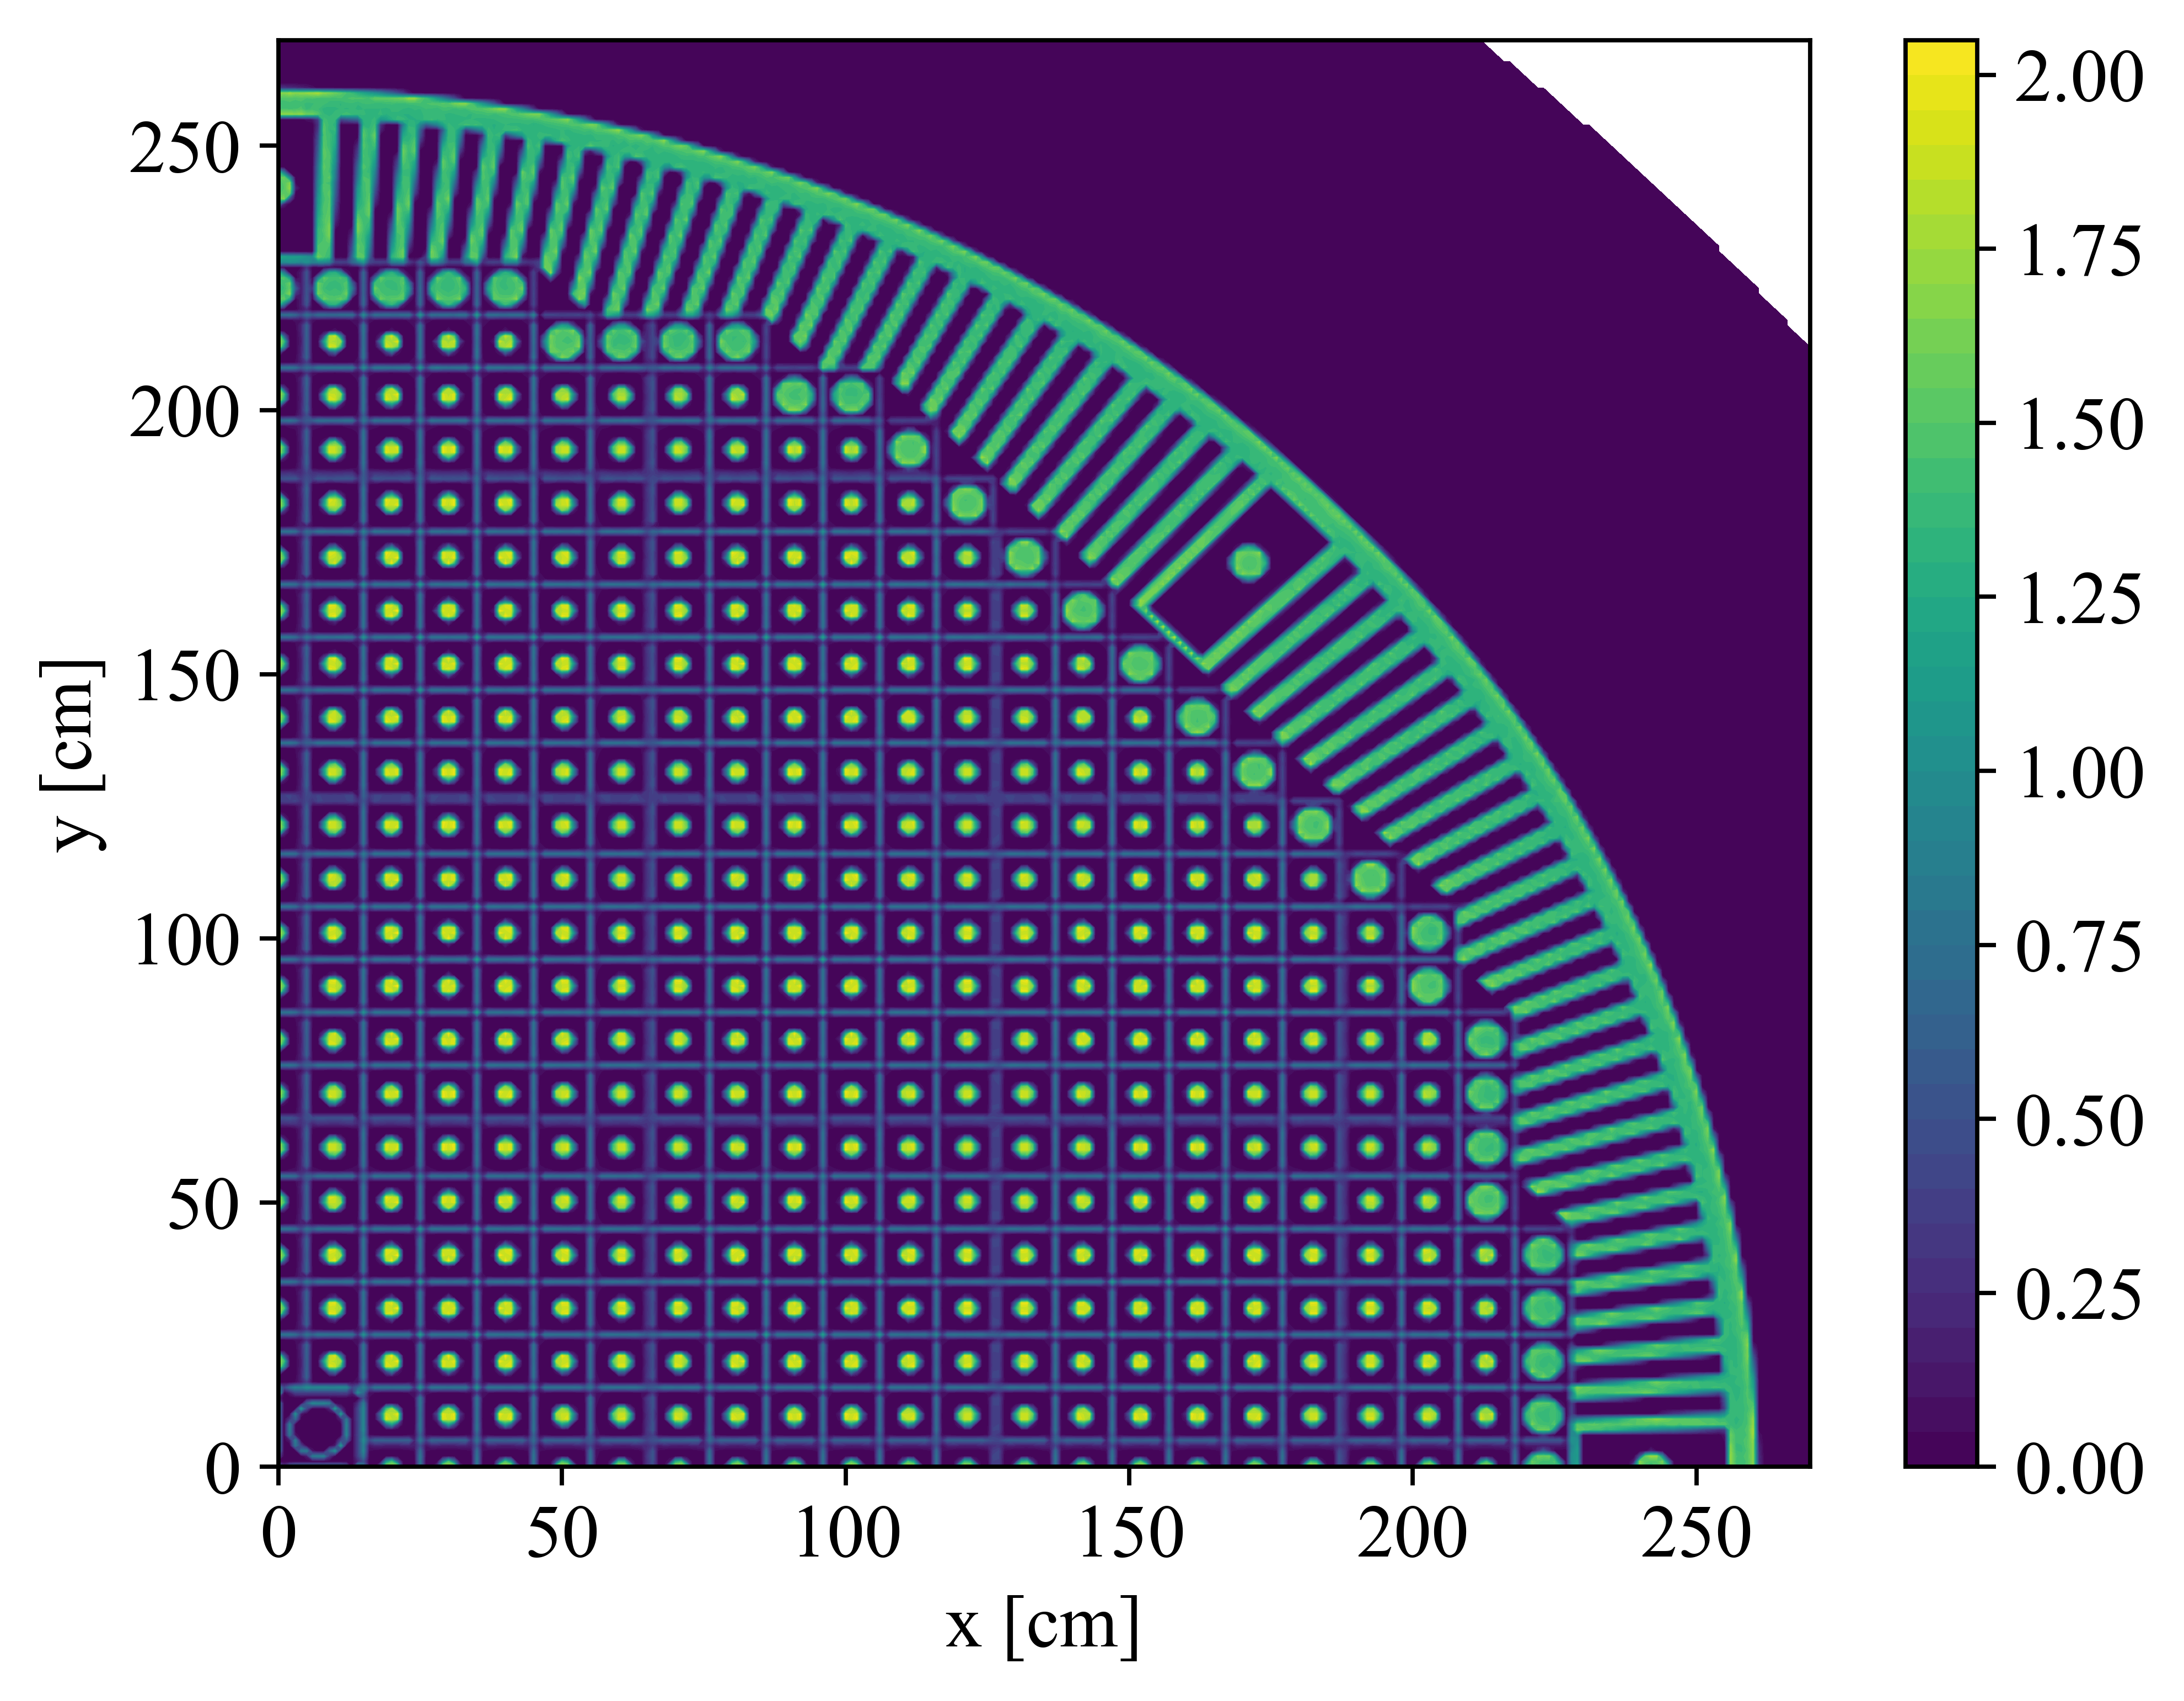
\includegraphics[width=\textwidth]{breeding_distribution_eq.png} 
    \end{center}
	\caption{$^{232}$Th neutron capture reaction rate normalized by total flux for both initial and equilibrium fuel salt composition.}
	\label{fig:breeding_den}
\end{figure}
\begin{figure}[htbp!]
    \begin{center}
		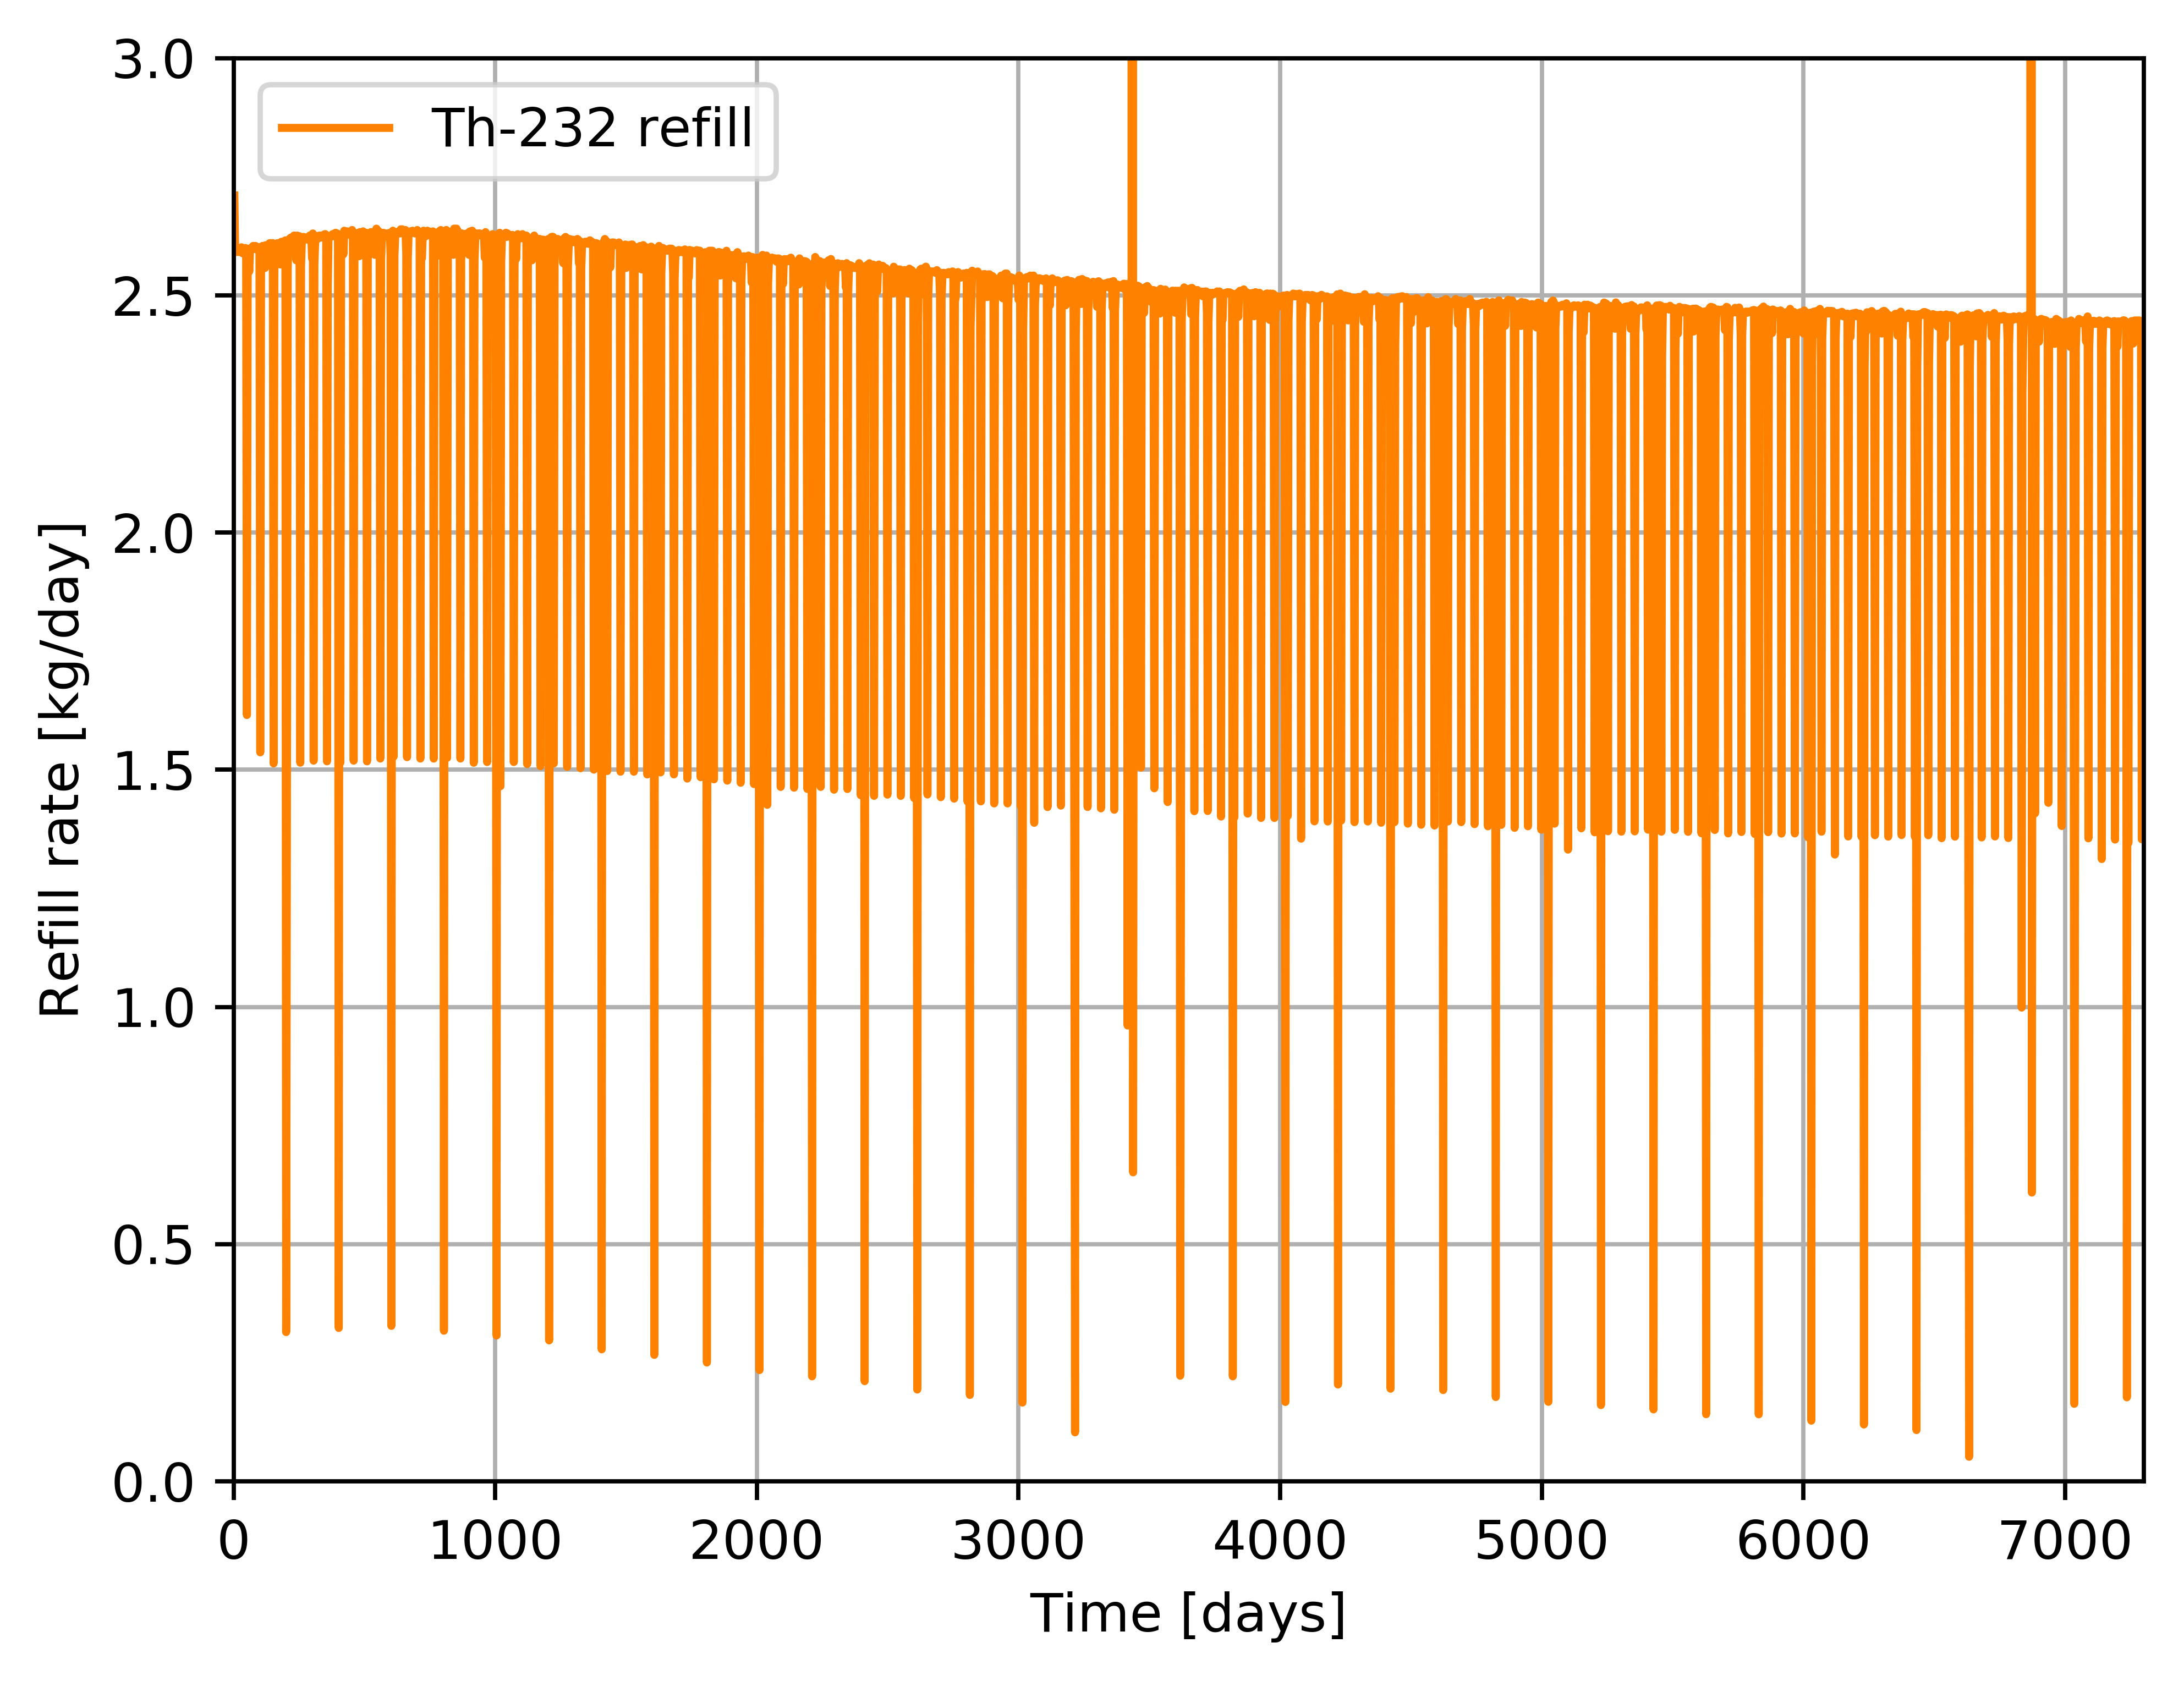
\includegraphics[width=\textwidth]{Th_refill_rate.png} 
    \end{center}
	\caption{$^{232}$Th feed rate over 60 years of Molten Salt Breeder Reactor operation.}
	\label{fig:th-rate}
\end{figure}
\begin{figure}[htbp!]
    \begin{center}
		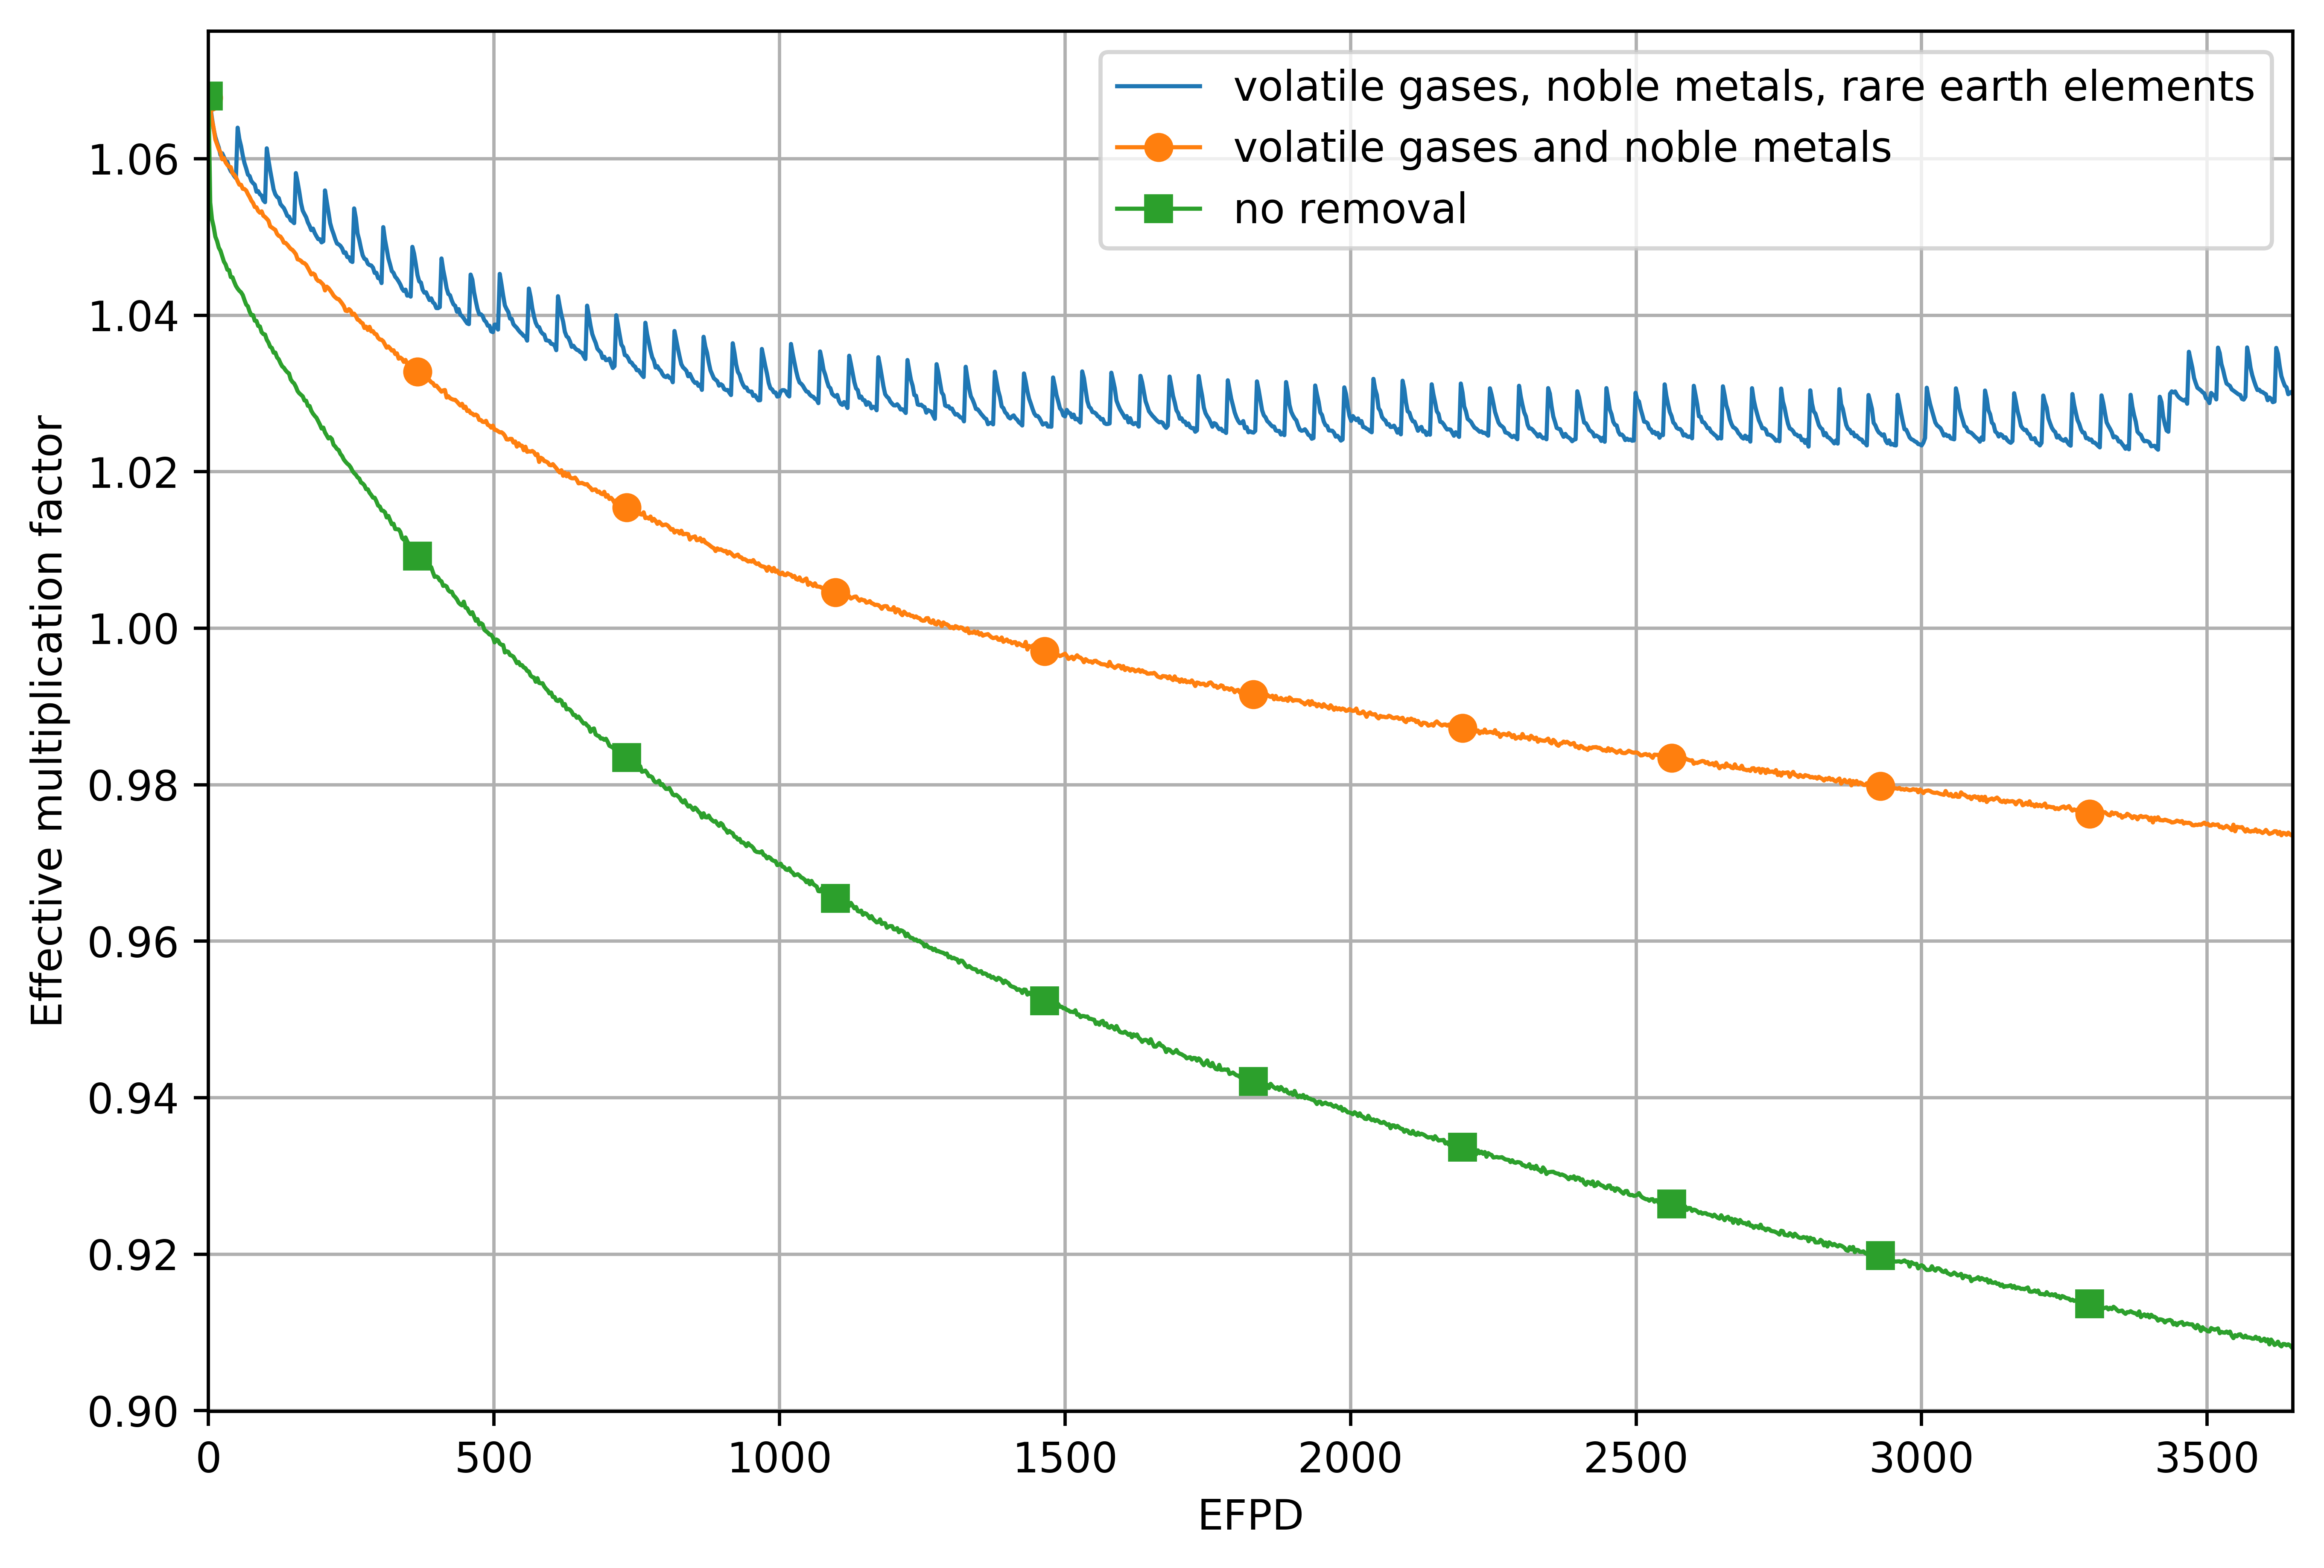
\includegraphics[width=\textwidth]{keff_rem_cases.png} 
    \end{center}
	\caption{Calculated effective multiplication factor for full-core model with removal of different fission product groups over 10 years of operation. The confidence interval $\pm\sigma$ is shaded.}
	\label{fig:fp-removal}
\end{figure}

\end{document}
